\documentclass[t,xcolor={svgnames,table}]{beamer}

\mode<presentation>
\usetheme{Warsaw}
\useoutertheme{infolines} 
\usepackage{natbib}
\usepackage{fontspec}
\usepackage{lmodern}
\usepackage{amsmath}
\usepackage{amsfonts}
\usepackage{bbm}
\usepackage{bm}
\usepackage[font=small,labelfont=bf]{caption} % Required for specifying captions to tables and figures
\usepackage{nicefrac}
\usepackage{color}
\usepackage{perpage}
\usepackage{multirow}
\usepackage{multicol}
\usepackage{adjustbox}
\usepackage{tikz}
\usepackage{tikz-dependency}
\usepackage{tikz-qtree}
\usepackage{tikz,pgfplots,pgfplotstable}
\usepackage{pgf}
\usepackage{collcell}
\usepackage{booktabs}
\usepackage{color,soul}
\usepackage[absolute,overlay]{textpos}

\graphicspath{{figures/}}

\usetikzlibrary{arrows.meta,graphs,graphs.standard,graphdrawing,quotes,shapes}
\usegdlibrary{layered,trees}

\tikzset{
  invisible/.style={opacity=0},
  visible on/.style={alt={#1{}{invisible}}},
  alt/.code args={<#1>#2#3}{%
    \alt<#1>{\pgfkeysalso{#2}}{\pgfkeysalso{#3}} % \pgfkeysalso doesn't change the path
  },
}

\captionsetup{labelformat=empty}
\newcommand{\parser}[1]{TUPA\textsubscript{#1}}

\newfontfamily\hebfont[Script=Hebrew, Scale=MatchUppercase]{FreeSans}
\newcommand{\heb}[1]{\bgroup\textdir TRT\hebfont #1\egroup}

\newcommand{\ucca}[1]{\textcolor{gray}{\textbf{\textsf{#1}}}}
\newcommand{\sst}[1]{\textsc{#1}}
\newcommand{\lexcat}[1]{\textsl{#1}}

\definecolor{orange}{rgb}{1,0.5,0}
\definecolor{mdgreen}{rgb}{0.05,0.6,0.05}
\definecolor{Acolor}{HTML}{EC5D57} % poppy red
\definecolor{Pcolor}{HTML}{70BF41} % grass green
\definecolor{Scolor}{HTML}{51A7F9} % sky blue
\definecolor{Lcolor}{HTML}{B36AE2} % friendly purple
\definecolor{mdblue}{rgb}{0,0,0.7}
\definecolor{dkblue}{rgb}{0,0,0.5}
\definecolor{dkgray}{rgb}{0.3,0.3,0.3}
\definecolor{slate}{rgb}{0.25,0.25,0.4}
\definecolor{gray}{rgb}{0.5,0.5,0.5}
\definecolor{ltgray}{rgb}{0.7,0.7,0.7}
\definecolor{purple}{rgb}{0.7,0,1.0}
\definecolor{lavender}{rgb}{0.65,0.55,1.0}
\definecolor{lightblue}{rgb}{.90,.95,1}
\sethlcolor{lightblue}
\renewcommand<>{\hl}[1]{\only#2{\beameroriginal{\hl}}{#1}}
\definecolor{kugreen}{RGB}{50,93,61}
\definecolor{kugreenlys}{RGB}{132,158,139}
\definecolor{kugreenlyslys}{RGB}{173,190,177}
\definecolor{kugreenlyslyslys}{RGB}{214,223,216}
\definecolor{ku}{RGB}{144,26,30}
\definecolor{ku-yellow}{RGB}{255,249,25}
\definecolor{lightgreen}{RGB}{0,128,0}

\newcommand{\semitransp}[2][20]{\color{fg!#1}#2}

\makeatletter
\pgfdeclareshape{vector}{
      \inheritsavedanchors[from={rectangle}]
      \inheritbackgroundpath[from={rectangle}]
      \inheritanchorborder[from={rectangle}]
      \foreach \x in {center,north east,north west,north,south,south east,south west,east,west}{
        \inheritanchor[from={rectangle}]{\x}
      }

    \backgroundpath{
      \pgftransformshift{\pgfpoint{-16pt}{-4pt}}
          \draw[rounded corners=2pt] (0,0) rectangle (32pt,8pt);
    }

    \beforebackgroundpath{
      \draw[step=8pt,help lines,-] (8pt,.1pt) grid (24pt,7.9pt);
    }
}
\pgfdeclareshape{vector}{
      \inheritsavedanchors[from={rectangle}]
      \inheritbackgroundpath[from={rectangle}]
      \inheritanchorborder[from={rectangle}]
      \foreach \x in {center,north east,north west,north,south,south east,south west,east,west}{
        \inheritanchor[from={rectangle}]{\x}
      }

    \backgroundpath{
      \pgftransformshift{\pgfpoint{-16pt}{-4pt}}
          \draw[rounded corners=2pt] (0,0) rectangle (32pt,8pt);
    }

    \beforebackgroundpath{
      \draw[step=8pt,help lines,-] (8pt,.1pt) grid (24pt,7.9pt);
    }
}
\makeatother


% for confusion matrix
\newcommand{\ApplyGradient}[1]{%
  \pgfmathsetmacro{\PercentColor}{(#1-0)/63.88}%
  \pgfmathsetmacro{\PercentInverse}{ifthenelse(\PercentColor > 70, 0, 100)}%
  %\textcolor{black!\PercentColor}{#1}
  \edef\x{\noexpand\cellcolor{red!\PercentColor}}\x\textcolor{black!\PercentInverse}{#1}%
}
\newcolumntype{R}{>{\collectcell\ApplyGradient}{c}<{\endcollectcell}}

\MakePerPage{footnote}

% Outline slides
\AtBeginSection[]
{\begin{frame} \frametitle{Outline} \tableofcontents[currentsection,currentsubsection] \end{frame}}


\begin{document}


\title[]{Universal Meaning Representation Parsing}
\author{Daniel Hershcovich}
\date{ML Section \\ November 9, 2020}

\begin{frame}
\titlepage
\end{frame}

\begin{frame}
\frametitle{What can we do with Natural Language Processing?}
\onslide<2>{Machine translation:}
\begin{center}
\onslide<2,5>{
  \fbox{\heb{דניאל עבר לקופנהגן אחרי שסיים את הלימודים}}
}

\only<2,4>{
  \fbox{After graduation, Daniel moved to Copenhagen}
}
\only<3,5->{
  \fbox{After graduation, \underline{Daniel} moved to \underline{Copenhagen}}
}
\end{center}

\vspace{-7mm}
  
\only<3>{
  \vspace{-9mm}

  Named \\ entity \\ recognition:

  \hspace{54mm} $\downarrow$ \hspace{27mm} $\downarrow$

  \hspace{49mm} Person \hspace{17mm} Location
}

\only<4>{
  Text \\
  simplification:
}
  
\only<4->{
  \vspace{1mm}
  \begin{center}  
  \fbox{Daniel graduated. Then Daniel moved to Copenhagen.}
  \end{center}
}

\only<5->{
  Neural models require the right \textit{inductive bias}
  \citep{barrett-etal-2018-sequence}.

  \begin{center}
    \begin{tikzpicture}[->]
    \tikzstyle{main}=[circle, minimum size=7mm, draw=black!80, node distance=12mm]
    \foreach \i in {1,3,7,9} {
        \node[main, fill=white!100] (h\i) at (\i,0) {};
        \node[main, fill=white!100] (o\i) at (\i.5,2) {};
    }
    \node (h5) at (5.5,0) {$\ldots$};
    \node (o5) at (5.5,2) {$\ldots$};
    \foreach \current/\next in {1/3,3/5,5/7,7/9} {
        \path (h\current) edge (h\next);
        \path (o\current) edge (o\next);
    }
    \foreach \i in {1,3,7,9} {
      \foreach \j in {1,3,7,9} {
        \path[gray!50] (h\i) edge (o\j);
      }
    }
    \path [alt=<6>{red,line width=1pt}{}] (h1) edge (o7);
    \end{tikzpicture}
  \end{center}
}

\end{frame}

\begin{frame}
\frametitle{Structured Inductive Bias}
Symbolic relations between words or concepts.

\vfill

Example: {\color{DarkBlue}syntactic}/{\color{DarkRed}semantic} bi-lexical dependencies.

\vfill

    \begin{adjustbox}{center}
    \begin{dependency}[line width=1.5pt]
        \begin{deptext}[column sep=1.5em,ampersand replacement=\^,font=\rmfamily]
          After \^ graduation \^ , \^ Daniel \^ moved \^ to \^ Copenhagen \\
        \end{deptext}
        \depedge[edge below,draw=DarkRed,edge unit distance=3ex]{1}{2}{ARG2}
        \depedge[edge below,draw=DarkRed,edge unit distance=3ex]{5}{4}{ARG1}
        \depedge[edge below,draw=DarkRed,edge unit distance=2ex, edge end x offset=-2pt]{1}{5}{ARG1}
        \deproot[edge below,draw=DarkRed,edge unit distance=3ex]{5}{top}
        \depedge[edge below,draw=DarkRed,edge unit distance=4ex, edge start x offset=-1pt, edge end x offset=3pt]{5}{7}{ARG2}
        \depedge[edge below,draw=DarkRed,edge unit distance=3ex, edge end x offset=5pt]{6}{5}{ARG1}
        \depedge[edge below,draw=DarkRed,edge unit distance=3ex]{6}{7}{ARG2}
        \depedge[draw=DarkBlue,edge unit distance=3ex]{2}{1}{case}
        \depedge[draw=DarkBlue,edge unit distance=3ex]{2}{3}{punct}
        \depedge[draw=DarkBlue,edge unit distance=3ex]{5}{4}{nsubj}
        \depedge[draw=DarkBlue,edge unit distance=3ex, edge end x offset=-2pt]{5}{2}{obl}
        \depedge[draw=DarkBlue,edge unit distance=3ex]{7}{6}{case}
        \deproot[draw=DarkBlue,edge unit distance=4ex]{5}{root}
        \depedge[draw=DarkBlue,edge unit distance=4ex]{5}{7}{obl}
    \end{dependency}    
    
    \end{adjustbox}
\end{frame}

\begin{frame}
    \frametitle{Meaning Representation}
Abstract away from detail that does not affect meaning:
\begin{center}    
    \fbox{\textrm{graduation}} $\approx$ \fbox{\textrm{graduated}}
    $\approx$ \fbox{\heb{סיים את הלימודים}} $\approx$ \fbox{\textrm{Abschluss}}
\end{center}

\pause\vfill

But capture useful distinctions, such as:
\vfill

\begin{minipage}{.38\textwidth}
\begin{itemize}
\item {\only<2>{\color{red}}Scenes and participants}
\item {\only<3>{\color{red}}Scene linkage}
\item {\only<4>{\color{red}}Multi-word chunking}
\end{itemize}
\end{minipage}
\begin{minipage}{.58\textwidth}\scalebox{.8}{
            \begin{tikzpicture}[level distance=21mm, sibling distance=1mm,
                every node/.append style={font=\rmfamily},
            	every circle node/.append style={fill=Indigo}]
                \begin{scope}[frontier/.style={distance from root=56mm},
                    edge from parent/.append style={nodes={font=\scriptsize}}]
                \Tree [.\node [circle] (root u) {};
                  \edge node[auto=right]{L}; \node[alt=<3>{text=red}{}] {Nach};
                  \edge node[auto=left]{H};
                  [.\node[circle](abschluss) {};
                    \edge node[auto=left]{P};
                    [.\node [circle] {};
                      \edge node[auto=right]{R}; \node {seinem};
                      \edge node[right]{C}; \node[alt=<2>{text=red}{}] (graduation) {Abschluss};
                    ]
                  ]
                  \edge node[auto=left]{H};
                  [.\node[circle]{};
                    \edge node[auto=left]{P};
                    [.\node[circle,xshift=8mm](zogum) {};
                      \edge node[auto=right]{}; \node[alt=<4>{text=red}{}] {zog};
                    ]
                    \edge node[right]{A}; \node[alt=<2>{text=red}{}] (Daniel) {Daniel};
                    \edge[draw=none]; \node[alt=<4>{text=red}{}] (um) {um};
                  ]
                ]
                \draw[dashed] (abschluss) to node[auto] {A} (Daniel);
                \draw (zogum.south) to node[left] {} (um);
                \end{scope}
            \end{tikzpicture}}
\end{minipage}\end{frame}


\section{UCCA}

\begin{frame}
\frametitle{Universal Conceptual Cognitive Annotation (UCCA)}
Supports rapid and intuitive annotation of linguistic semantic phenomena. \\
\only<1>{\citep{abend2013universal}}
\onslide<2->{
  Cross-linguistically applicable and stable \citep{sulem2015conceptual}.
}

\vfill

\begin{adjustbox}{center}
            \begin{tikzpicture}[level distance=7mm, sibling distance=6mm,
                every node/.append style={font=\rmfamily},
            	every circle node/.append style={fill=Indigo}]
                \begin{scope}[frontier/.style={distance from root=23mm},
                    edge from parent path={(\tikzparentnode.center)
                	.. controls +(0,-.25) and +(0,.25) .. (\tikzchildnode.north)},
                    edge from parent/.append style={nodes={font=\scriptsize}}]
                \Tree [.\node [circle] (root u) {};
                  \edge node [auto=right]{L}; \node (After u) {After};
                  \edge node[auto=left]{H};
                  [.\node [circle,xshift=8mm](graduation Daniel u) {};
                    \edge node[auto=right]{P}; \node (graduation u) {graduation};
                  ]
                  \edge node[auto=left]{H};
                  [.\node [circle](Daniel moved to Copenhagen u) {};
                    \edge node[auto=right]{A}; \node (Daniel u) {Daniel};
                    \edge node[auto=left]{P}; \node (moved u) {moved};
                    \edge node[auto=left]{A};
                    [.\node [circle](to Copenhagen u) {};
                      \edge node[auto=right]{R}; \node (to u) {to};
                      \edge node[auto=left]{C}; \node (Copenhagen u) {Copenhagen};
                    ]
                  ]
                ]
                \draw[dashed] (graduation Daniel u) to node[auto,style={font=\scriptsize}] {A} (Daniel u);
                \end{scope}
                \onslide<2->{
                  \begin{scope}[xshift=2cm,yshift=-58mm,grow'=up,level distance=9mm,
                      sibling distance=4mm, frontier/.style={distance from root=19mm},
                      edge from parent path={(\tikzparentnode.center) ..
                      controls +(0,.25) and +(0,-.25) .. (\tikzchildnode.south)},
                      edge from parent/.append style={nodes={font=\scriptsize}}]
                  \Tree [.\node [circle] (rootd) {};
                    \edge node[auto=left]{H};
                    [.\node [circle,xshift=-5mm] (Daniel siyem et halimudim d) {};
                      \edge node[auto=left]{P}; \node (halimudim d) {\heb{הלימודים}};
                      \edge node[auto=left]{F}; \node (et d) {\heb{את}};
                      \edge node[auto=right]{D}; \node (siyem d) {\heb{שסיים}};
                    ]
                    \edge node [auto=left,anchor=south east]{L}; \node (ahrei d) {\heb{אחרי}};
                    \edge node[auto=right]{H};
                    [.\node [circle] (hu avar lecopenhagen d) {};
                      \edge node[auto=left,anchor=south east]{A}; \node (lecopenhagen d) {\heb{לקופנהגן}};
                      \edge node[auto=left]{P}; \node (avar d) {\heb{עבר}};
                      \edge node[auto=right]{A}; \node (Daniel d) {\heb{דניאל}};
                    ]
                  ]
                  \draw[dashed] (Daniel siyem et halimudim d) to[out=-15,in=-150] node[above,style={font=\scriptsize}] {A} (Daniel d);
                  \end{scope}
                }\onslide<3>{
                  \begin{scope}[dashed,thick]
                    \draw[DarkRed] (After u) to[out=-45,in=135] (ahrei d);
                    \draw[DarkGreen] (graduation u) to[out=-90,in=100] (Daniel siyem et halimudim d);
                    \draw[DarkBlue] (Daniel u) -- (Daniel d);
                    \draw[orange] (moved u) to[out=-30,in=90] (avar d);
                    \draw[magenta] (to Copenhagen u) to[out=-90,in=70] (lecopenhagen d);
                  \end{scope}
                }
            \end{tikzpicture}
\end{adjustbox}
\end{frame}


\begin{frame}
\frametitle{UCCA Applications}
Semantics-based \textbf{evaluation} of
  \begin{itemize}
    \item Machine translation \citep{birch2016hume}.
    \item Text simplification \citep{sulem2018semantic}.
    \item {\only<2>{\color{red}}Grammatical error correction} \citep{choshen2018reference}.
  \end{itemize}

{\only<3>{\color{red}}Sentence splitting for text simplification} \citep{sulem2018simple}.

\pause

    \begin{minipage}{0.47\textwidth}
        \centering
        \scalebox{.9}{
                \begin{tikzpicture}[sibling distance=3mm, level distance=7mm,
                every node/.append style={font=\rmfamily},
            	every circle node/.append style={fill=black}]
                \begin{scope}[frontier/.style={distance from root=15mm},
            	edge from parent path={(\tikzparentnode.center) ..
                    controls +(0,-.25) and +(0,.25) .. (\tikzchildnode.north)}]
                \Tree [.\node [circle] (rootu) {};
                \edge node [auto=right]{}; \node (Heu) {He};
                \edge node[auto=right down]{}; \node (gve) {gve};
                \edge node[auto=right]{};
                [.\node [circle](an appleu) {};
                \edge node[auto=right]{}; \node (anu) {an};
                \edge node[auto=left]{}; \node (appleu) {apple};
                ]
                \edge node[auto=left]{};
                [.\node [circle](for daniel) {};
                \edge node[auto=right]{};\node (for) {for};
                \edge node[auto=left]{}; \node (daniel) {her};
                ]]
                \end{scope}
                \begin{scope}[yshift=-41mm,grow'=up,
                  frontier/.style={distance from root=12mm},
                  edge from parent path={(\tikzparentnode.center) ..
                  controls +(0,.25) and +(0,-.25) .. (\tikzchildnode.south)}]
                \Tree [.\node [circle] (rootd) {};
                \edge node [auto=left]{}; \node (Hed) {He};
                \edge node[auto=right]{}; \node (gave) {gave};
                \edge node[auto=right]{};\node (Daniel) {her};
                \edge node[auto=right]{};
                [.\node [circle] (an appled) {};
                \edge node[auto=left]{}; \node (and) {an};
                \edge node[auto=right]{}; \node (appled) {apple};
                ]
                ]
                \end{scope}
                \begin{scope}[dashed]
                \draw (Heu) -- (Hed);
                \draw (gve) -- (gave);
                \draw (Daniel) -- (daniel);
                \draw (anu) -- (and);
                \draw (appleu) -- (appled);
                \end{scope}
                \end{tikzpicture}
        }
    \end{minipage}
\pause
    \begin{minipage}{0.43\textwidth}
        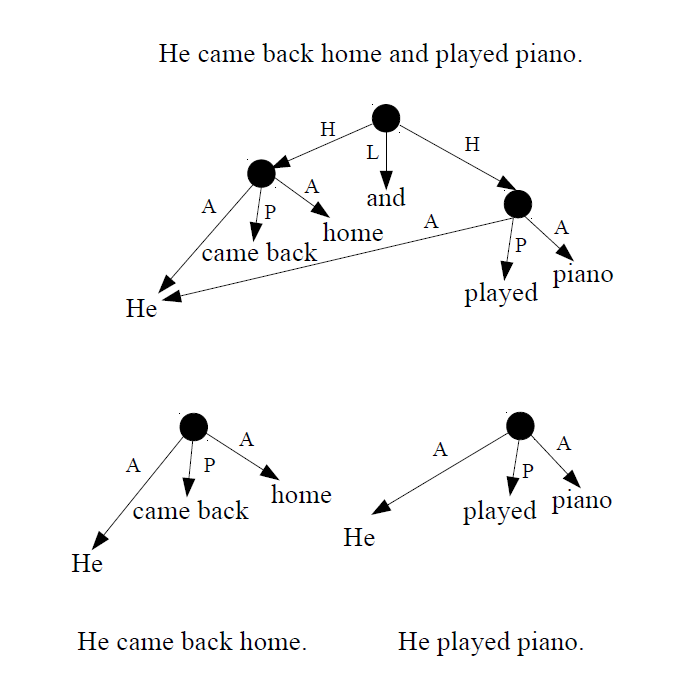
\includegraphics[width=1.2\textwidth,height=48mm]{ucca_simplification}  
    \end{minipage}

\end{frame}

\begin{frame}
\frametitle{UCCA Data}
\begin{itemize}
 \item English Wikipedia articles.
 \item English-French-German \textit{Twenty Thousand Leagues Under the Sea}.
 \item English Web Treebank reviews.
\end{itemize}

\vfill
\begin{center}
  \begin{minipage}{.26\textwidth}
\includegraphics[width=\textwidth]{wikipedia.png}\end{minipage}
  \begin{minipage}{.3\textwidth}
\includegraphics[width=\textwidth]{squid.jpg}\end{minipage}
  \begin{minipage}{.3\textwidth}
\includegraphics[width=\textwidth]{five-stars.png}\end{minipage}
\end{center}
\end{frame}


\begin{frame}
\frametitle{TUPA: Transition-based UCCA Parser}

Parses text $w_1 \ldots w_n$ to graph $G$ incrementally by applying transitions to the parser state,
consisting of: stack, buffer and constructed graph \citep*{hershcovich2017a}.

\pause
\vfill
Initial state:
\scalebox{.9}{
\begin{tikzpicture}[xscale=1.4,every node/.append style={font=\rmfamily,
                    anchor=west,text height=.6ex,text depth=0}, circle]
    \draw[xstep=1,ystep=.5,color=gray] (-.01,0) grid (1,.5);
    \node[style={font=\sffamily}] at (-.1,.8) {stack};
    \node[fill=black] at (.3,.25) {};
    \draw[xstep=1,ystep=.5,color=gray] (2,0) grid (9,.5);
    \node[style={font=\sffamily}] at (8,.8) {buffer};
    \node at (2,.2) {\small They};
    \node at (3,.2) {\small thought};
    \node at (4,.2) {\small about};
    \node at (5,.2) {\small taking};
    \node at (6,.2) {\small a};
    \node at (7,.2) {\small short};
    \node at (8,.2) {\small break};
\end{tikzpicture}}

\vfill
\pause
\parser{} transitions:

\{\textsc{Shift, Reduce, {\color{blue}Node$_X$}, Left-Edge$_X$, Right-Edge$_X$,}\\
\hspace{5mm}\textsc{{\color{orange}Left-Remote$_X$}, {\color{orange}Right-Remote$_X$}, {\color{red}Swap}, Finish}\}
\end{frame}

\begin{frame}
\frametitle{Training}
An \textit{oracle} provides the transition sequence given the correct graph:

\vfill
\centering
\scalebox{.8}{
\begin{tikzpicture}[level distance=15mm, sibling distance=2cm, ->, thick,
    every node/.append style={font=\rmfamily},
    edge from parent/.append style={nodes={font=\scriptsize}},
    edge from parent path={(\tikzparentnode.center) -- (\tikzchildnode.north)}]
    \node(ROOT)[fill=black, circle] at (3,0) {}
      child {node (They) {They} edge from parent node [left] {A}}
      child {node (thought) {thought} edge from parent node [left] {P}}
      child {node (abouttakingashortbreak) [fill=blue, circle] {} 
      { 
        child {node (to) {about} edge from parent node [right] {R}}
        child {node (takingabreak) [fill=red, circle] {}
        {
          child {node (take) {taking} edge from parent node [above] {F}}      
          child {node (a) {a} edge from parent node [right] {F}} 
          child {node (short) {short} edge from parent [draw=none]}
          child {node (break) {break} edge from parent node [above] {C}}  
        } edge from parent [draw=none]}
      } edge from parent [draw=none]}
      ;
    \draw(abouttakingashortbreak) to node [left] {\scriptsize P} (takingabreak); 
    \draw(ROOT) to node [left] {A} (abouttakingashortbreak);
    \draw[bend left,dashed] (abouttakingashortbreak) to node [auto] {A} (They);
    \draw[bend left] (abouttakingashortbreak) to node [auto] {\scriptsize D} (short);
\end{tikzpicture}}
\[\Downarrow\]
\begin{flushleft}
\footnotesize
\textsc{Shift}, \textsc{Right-Edge$_A$}, \textsc{Shift}, \textsc{Swap}, \textsc{Right-Edge$_P$}, \textsc{Reduce}, \textsc{Shift}, \textsc{Shift}, \textsc{Node$_R$}, \textsc{Reduce}, \textsc{Left-Remote$_A$}, \textsc{Shift}, \textsc{Shift}, \textsc{Node$_C$}, \textsc{Reduce}, \textsc{Shift}, \textsc{Right-Edge$_P$}, \textsc{Shift}, \textsc{Right-Edge$_F$}, \textsc{Reduce}, \textsc{Shift}, \textsc{Swap}, \textsc{Right-Edge$_D$}, \textsc{Reduce}, \textsc{Swap}, \textsc{Right-Edge$_A$}, \textsc{Reduce}, \textsc{Reduce}, \textsc{Shift}, \textsc{Reduce}, \textsc{Shift}, \textsc{Right-Edge$_C$}, \textsc{Finish}
\end{flushleft}
\end{frame}

\begin{frame}
\frametitle{\parser{} Model}
Learns to greedily predict transition based on current state.

\centering
\fbox{\scalebox{.65}{
\begin{minipage}{.6\textwidth}
\begin{tikzpicture}[xscale=1.3,every node/.append style={font=\rmfamily}]
    \node[anchor=west,style={font=\sffamily}] at (-1,.25){stack};
    \draw[xstep=1,ystep=.5,color=gray] (-.01,0) grid (4,.5);
    \node[fill=black, circle] at (.5,.25) {};
    \node[fill=blue, circle] at (2.5,.25) {};
    \node[anchor=west] at (1,.25) {\small They};
    \node[anchor=west] at (3,.25) {\small taking};
\end{tikzpicture}

\vspace{1cm}
\begin{tikzpicture}[xscale=1.3,every node/.append style={font=\rmfamily}]
    \node[anchor=west,style={font=\sffamily}] at (-1,.25){buffer};
    \draw[xstep=1,ystep=.5,color=gray] (-.01,0) grid (4,.5);
    \node[fill=red, circle] at (.5,.25) {};
    \node[anchor=west] at (1,.25) {\small a};
    \node[anchor=west] at (2,.25) {\small short};
    \node[anchor=west] at (3,.25) {\small break};
\end{tikzpicture}
\end{minipage}
\begin{minipage}{.4\textwidth}
\scalebox{.65}{
\begin{tikzpicture}[xscale=1.5,level distance=1cm, sibling distance=12mm, ->,
    every node/.append style={font=\rmfamily,
                    anchor=west,text height=.6ex,text depth=0},
    edge from parent/.append style={nodes={font=\scriptsize}},
    edge from parent path={(\tikzparentnode.center) -- (\tikzchildnode.north)}]
    \node[anchor=west,style={font=\sffamily}] at (3,0) {graph};
    \draw[color=gray] (.2,.3) rectangle (3.9,-3.2);
    \node(ROOT)[fill=black, circle] at (1.2,0) {}
      child {node (They) {They} edge from parent node [left] {A}}
      child {node {thought} edge from parent node [left] {P}}
      child {node (abouttakingashortbreak) [fill=blue, circle] {}
      {
        child {node {about} edge from parent node [left] {R}}
        child {node (takingabreak) [fill=red, circle] {}
        {
          child {node {taking} edge from parent node [above] {F}}
          child [opacity=0] {node {a} edge from parent node [right] {F}}
          child [opacity=0] {node (short) {short} edge from parent [draw=none]}
          child [opacity=0] {node {break} edge from parent node [right] {C}}
        } edge from parent [draw=none]}
      } edge from parent [draw=none]}
      ;
\end{tikzpicture}
}
\end{minipage}
}}

\scalebox{.65}{
\begin{tikzpicture}[->,every node/.append style={anchor=north,text height=2ex,text depth=0}]
    \tiny
    \tikzstyle{main}=[circle, minimum size=7mm, draw=black!80, node distance=12mm]
    \foreach \i/\word in {1/{They},3/{thought},5/{about},7/{taking},9/{a},11/{short},13/{break}} {
        \node (x\i) at (\i,-1.3) {\Large\textrm\word};
        \node[main, fill=white!100] (h\i) at (\i,0) {LSTM};
        \path (x\i) edge (h\i);
        \node[main, fill=white!100] (i\i) at (\i.5,.8) {LSTM};
        \path (x\i) edge [bend right] (i\i);
        \node[main, fill=white!100] (l\i) at (\i.5,2.3) {LSTM};
        \path (h\i) edge [bend left] (l\i);
        \path (i\i) edge (l\i);
        \node[main, fill=white!100] (k\i) at (\i,3.1) {LSTM};
        \path (i\i) edge [bend left] (k\i);
        \path (h\i) edge [bend left] (k\i);
    }
    \foreach \current/\next in {1/3,3/5,5/7,7/9,9/11,11/13} {
        \path (h\current) edge (h\next);
        \path (i\next) edge (i\current);
        \path (l\current) edge (l\next);
        \path (k\next) edge (k\current);
    }
    \node[main, fill=white!100] (mlp) at (7,4.6) {MLP};
    \foreach \i in {1,5,7,9} {
        \path (l\i) edge (mlp);
        \path (k\i) edge (mlp);
    }
    \coordinate (state) at (10.5,6.5);
    \path (state) edge [bend left] (mlp);
    \node (transition) at (7,5.8) {\large\textsc{Node}$_C$};
    \path (mlp) edge (transition);
\end{tikzpicture}
}
\end{frame}

\begin{frame}{Refining Implicit Argument Annotation for UCCA}
\citep*{cui-hershcovich-2020-refining}
\hfill

\includegraphics[width=.15\textwidth]{ruixiang}
\begin{center}
\scalebox{.7}{
\begin{tikzpicture}[->,level distance=1.55cm,
  level 1/.style={sibling distance=4cm},
  level 2/.style={sibling distance=20mm},
  level 3/.style={sibling distance=20mm},
  every circle node/.append style={fill=black},
  every node/.append style={text height=1ex,text depth=0}]
  \tikzstyle{word} = [font=\rmfamily,color=black]
  \node (1_1) [circle] {}
  {
  child {node (1_2) [circle] {}
    {
    child {node (1_16) [word] {\textbf{IMP}$_\text{Non-specific}$}  edge from parent node[midway, fill=white]  {A}}
    child {node (1_8) [word] {Have}  edge from parent node[midway, fill=white]  {D}}
    child {node (1_9) [circle] {}
      {
      child {node (1_13) [word] {a}  edge from parent node[midway, fill=white]  {F}}
      child {node (1_12) [word] {real}  edge from parent [white]}
      child {node (1_14) [word] {mechanic}  edge from parent node[midway, fill=white]  {C}}
      } edge from parent node[midway, fill=white]  {A}}
    child {node (1_10) [word] {check}  edge from parent node[midway, fill=white]  {P}}
    } edge from parent node[midway, fill=white]  {H}}
  child {node (1_3) [word] {before}  edge from parent node[midway, fill=white]  {L}}
  child {node (1_4) [circle] {}
    {
    child {node (1_6) [word] {you}  edge from parent node[midway, fill=white]  {A}}
    child {node (1_7) [word] {leave}  edge from parent node[midway, fill=white]  {P}}
    child {node (1_17) [word] {\textbf{IMP}$_\text{Non-specific}$}  edge from parent node[midway, fill=white]  {A}}
    } edge from parent node[midway, fill=white]  {H}}
  };
  \draw[dashed,->] (1_2) to node [midway, fill=white] {A} (1_6);
  \draw[bend right,->] (1_2) to[out=-20, in=180] node [midway, fill=white] {D} (1_12);
\end{tikzpicture}}
\end{center}
\end{frame}

\begin{frame}{Refining Implicit Argument Annotation for UCCA}
\begin{center}
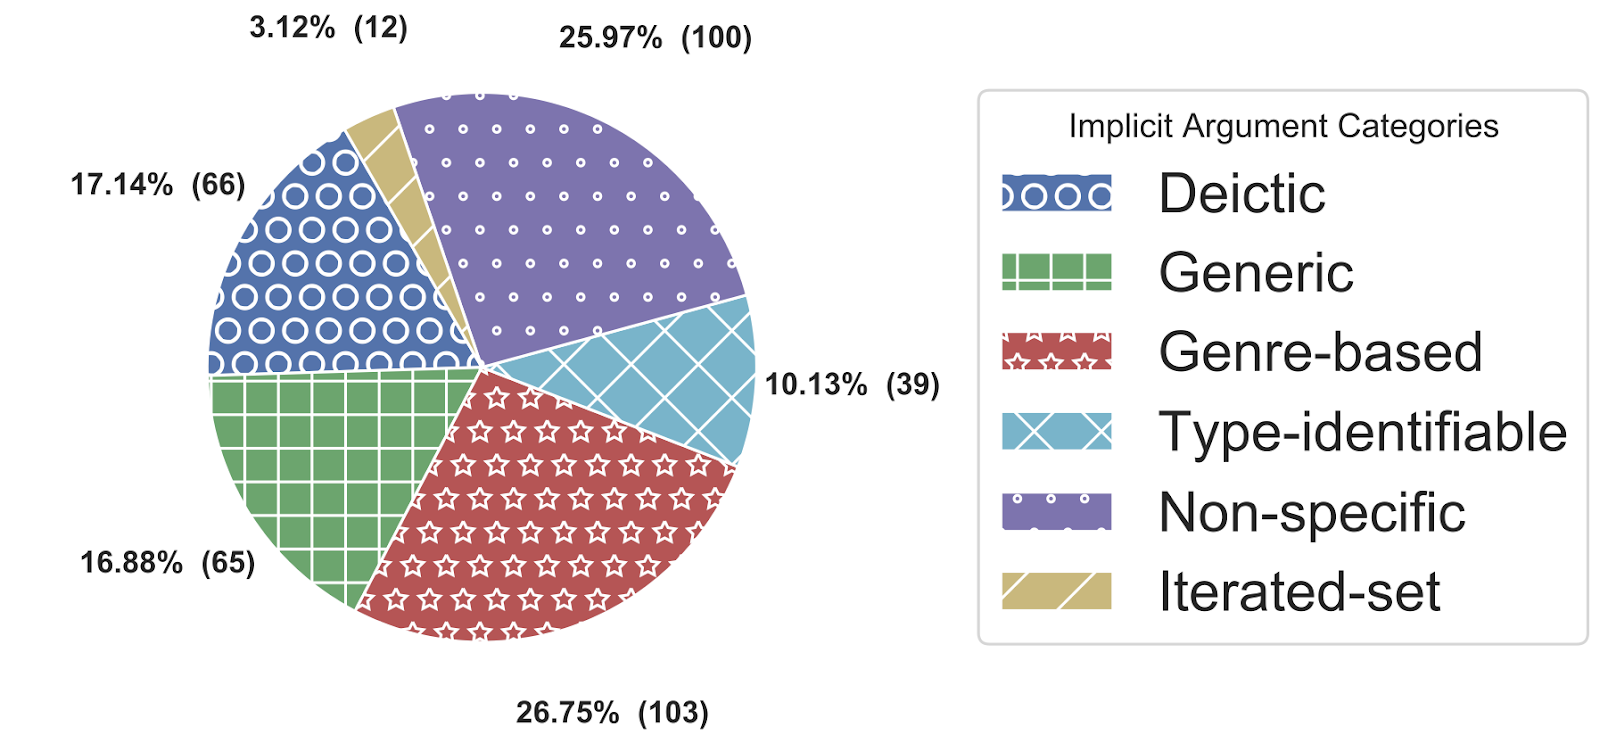
\includegraphics[width=.8\textwidth]{implicit_pie}
\end{center}
\end{frame}


\section{Parsing}


\begin{frame}
    \frametitle{Meaning Representations}

      \begin{flushright}
        \scalebox{.6}{
\begin{tikzpicture}[level distance=2cm, sibling distance=25mm, ->, draw=Indigo, thick]
    \node[font=\bf\sffamily\Huge,Indigo] at (-3,0) {UCCA};
    \node (ROOT) [fill=Indigo, circle] {}
      child {node (After) {After} edge from parent node[left] {L\;}}
      child {node (graduation) [fill=Indigo, circle] {}
      {
        child {node {graduation} edge from parent node[left] {P}}
      } edge from parent node[left] {H} }
      child {node {,} edge from parent node[right] {U}}
      child {node (moved) [fill=Indigo, circle] {}
      {
        child {node (Daniel) {Daniel} edge from parent node[left] {A}}
        child {node {moved} edge from parent node[left] {P}}
        child {node [fill=Indigo, circle] {}
        {
          child {node {to} edge from parent node[left] {R}}
          child {node {Copenhagen} edge from parent node[left] {C}}
        } edge from parent node[left] {A} }
      } edge from parent node[right] {H} }
      ;
    \draw[dashed,->] (graduation) to node [auto] {A} (Daniel);
\end{tikzpicture}
        }
      \end{flushright}
    
    \vspace{-23mm}
    
    \scalebox{.6}{
\begin{tikzpicture}[thick]
\node[font=\bf\sffamily\Huge,DarkGreen] at (0,6) {AMR};
\graph[layered layout, sibling distance=4cm, layer distance=2cm, nodes={ellipse,draw=DarkGreen}, edges={nodes={sloped}, DarkGreen}]{
a4 Copenhagen[as={Copenhagen}];
a2 Daniel[as={Daniel}];
a1[as={person}];
a0[as={move-01}];
a3[as={city}];
a2[as={name}];
a5[as={after}];
a4[as={name}];
a6[as={graduate-01}];

a1 ->  ["name"' above] a2;
a0 ->  ["ARG0"' above] a1;
a0 ->  ["ARG2"' above] a3;
a0 ->  ["time"' above] a5;
a3 ->  ["name"' above] a4;
a2 ->  ["op1"' above] a2 Daniel;
a5 ->  ["op1"' above] a6;
a4 ->  ["op1"' above] a4 Copenhagen;
};
\draw[->, above, DarkGreen] (a6) to node[sloped] {ARG0} (a1);
\end{tikzpicture}
      }
    \vspace{-15mm}
    
    \begin{flushright}
    \begin{minipage}{.01\textwidth}
      \begin{tikzpicture}
        \node[font=\bf\sffamily\Large,DarkRed] {DM};
      \end{tikzpicture}
    \end{minipage}
    \begin{minipage}{.6\textwidth}
        \rmfamily
        \scalebox{.7}{
\begin{dependency}[theme=simple,edge style={-{Latex[length=2mm]}, color=DarkRed},
            text only label, label style={above, color=DarkRed, font=\bf\ttfamily}, font=\small, thick]
    \begin{deptext}[column sep=1em,ampersand replacement=\^]
	After \^ graduation \^ , \^ Daniel \^ moved \^ to \^ Copenhagen \\
    \end{deptext}
    \deproot{5}{top}
    \depedge{1}{2}{ARG2}
    \depedge{1}{5}{ARG1}
    \depedge{5}{4}{ARG1}
    \depedge{6}{5}{ARG1}
    \depedge{6}{7}{ARG2}
\end{dependency}
    }
    \end{minipage}
    \end{flushright}
\end{frame}


\begin{frame}
\frametitle{Syntactic Representations}
    {\color{DarkBlue}\bf\sffamily\Large UD} (Universal Dependencies)
    
    \begin{center}
    \rmfamily
    \begin{dependency}[text only label, edge style={-{Latex[length=2mm]}, color=DarkBlue}, thick,
                       label style={above, color=DarkBlue, font=\bf\ttfamily}, font=\small]
    \begin{deptext}[column sep=.8em,ampersand replacement=\^]
    After \^ graduation \^ , \^ Daniel \^ moved \^ to \^ Copenhagen \\
    \end{deptext}
        \depedge{2}{1}{case}
        \depedge{2}{3}{punct}
        \depedge{5}{4}{nsubj}
        \depedge[edge end x offset=-2pt]{5}{2}{obl}
        \depedge{7}{6}{case}
        \deproot[edge unit distance=2.5ex]{5}{root}
        \depedge{5}{7}{obl}
    \end{dependency}
    \end{center}
\end{frame}

\begin{frame}
    \frametitle{Data}
    \fbox{UCCA training data is scarce}
    \begin{center}
    \begin{minipage}{.15\textwidth}
      (English)
    \end{minipage}
    \begin{minipage}{.7\textwidth}
    \pgfplotstableread[row sep=\\,col sep=&]{
    	corpus & total \\
        \color{DarkBlue} UD & 35791 \\
        \color{DarkRed} DM & 33964 \\
        \color{DarkGreen} AMR & 36521 \\
        \color{Indigo} UCCA & 5141 \\
        }\english
        \begin{tikzpicture}
        \begin{axis}[
        xbar stacked,
        width=10cm,
        height=39mm,
        xmin=0,
        xmax=60000,
        xtick=\empty,
        ytick=data,
        yticklabels from table={\english}{corpus},
        axis x line=none,
        ]
        \addplot [fill=Navy, point meta=explicit symbolic,
        nodes near coords align={anchor=west}] table [x=total,y expr=\coordindex,meta=total] {\english};
        \end{axis}
        \end{tikzpicture}
    \end{minipage}
    \end{center}
    
    \pause
    \vfill
    
    \begin{flushright}
        \fbox{and domains are limited.}
    \end{flushright}
    \begin{center}
    \begin{tabular}{llll}
        \color{Indigo} UCCA  & \color{DarkGreen} AMR  & \color{DarkRed} DM  & \color{NavyBlue} UD  \\
    	Wikipedia & blogs & news & blogs \\ books & news && news \\ reviews & emails && emails \\ & reviews && reviews \\ &&& Q\&A
    \end{tabular}
    \end{center}
\end{frame}

\def\convertedudgraduation{
  \begin{tikzpicture}[level distance=15mm, ->, draw=DarkBlue, thick,
      every node/.append style={sloped,anchor=south,auto=false,font=\scriptsize},
      level 1/.style={sibling distance=16mm},
      level 2/.style={sibling distance=13mm},
      edge from parent path={(\tikzparentnode.center) -- (\tikzchildnode.north)}]
    \tikzstyle{word} = [font=\rmfamily,color=black]
    \node (ROOT) [fill=DarkBlue,circle] {}
      child {node (after) [fill=DarkBlue,circle] {}
      {
        child {node [word] {After{\color{white}g}\quad\quad} edge from parent node {case}}
        child {node [word] {\quad graduation\quad\quad} edge from parent node {head}}
      } edge from parent node {obl}}
      child {node {}
      {
        child {node [word] (comma) {\quad,{\color{white}g}} edge from parent [draw=none]}
      } edge from parent [draw=none]}
      child {node {}
      {
        child {node [word] (Daniel) {Daniel{\color{white}g}} edge from parent [draw=none]}
      } edge from parent [draw=none]}
      child {node {}
      {
        child {node [word] (moved) {moved{\color{white}g}} edge from parent [draw=none]}
      } edge from parent [draw=none]}
      child {node (to) [fill=DarkBlue,circle] {}
      {
          child {node [word] {to{\color{white}g}} edge from parent node {case}}
          child {node [word] {Copenhagen{\color{white}g}} edge from parent node {head}}
      } edge from parent node {obl}}
      ;
      \draw (ROOT) to node {punct} (comma);
      \draw (ROOT) to node {nsubj} (Daniel);
      \draw (ROOT) to node {head} (moved);
  \end{tikzpicture}
}


\begin{frame}
\frametitle{Conversion}

\begin{minipage}{.04\textwidth}
\vspace{4mm}
\color{DarkGreen} AMR\\
\vspace{13mm}
\color{DarkRed} DM\\
\vspace{14mm}
\color{DarkBlue} UD
\end{minipage}
\begin{minipage}{.45\textwidth}
  \centering
  \scalebox{.6}{
  \begin{tikzpicture}[->,draw=DarkGreen,
      every node/.append style={sloped,anchor=south,auto=false,font=\tiny},
      level 1/.style={level distance=14mm,sibling distance=26mm},
      level 2/.style={level distance=13mm},
      level 3/.style={level distance=12mm}]
    \node (ROOT) [draw=DarkGreen,ellipse] {move-01}
      child {node [draw=DarkGreen,ellipse] {city}
      {
        child {node [draw=DarkGreen,ellipse] {name}
        {
            child {node [draw=DarkGreen,ellipse] {"Copenhagen"} edge from parent node {op1} }
        } edge from parent node {name} }
      } edge from parent node {ARG2} }
      child {node [draw=DarkGreen,ellipse] {after}
      {
            child {node (graduation) [draw=DarkGreen,ellipse] {graduate-01} edge from parent node {op1} }
      } edge from parent node {time} }
      child {node (Daniel) [draw=DarkGreen,ellipse] {person}
      {
        child {node [draw=DarkGreen,ellipse] {name}
        {
            child {node [draw=DarkGreen,ellipse] {"Daniel"} edge from parent node {op1} }
        } edge from parent node {name} }
      } edge from parent node {ARG0} }
      ;
      \draw (graduation) to node {ARG0} (Daniel);
  \end{tikzpicture}
  }
  
  \vspace{5mm}
  \scalebox{.6}{
    \begin{dependency}[theme=simple,text only label, font=\small, edge style={color=DarkRed},
                       label style={above, color=DarkRed, font=\bf\ttfamily}]
    \begin{deptext}[column sep=.8em,ampersand replacement=\^]
    After \^ graduation \^ , \^ Daniel \^ moved \^ to \^ Copenhagen \\
    \end{deptext}
        \depedge{1}{2}{ARG2}
        \depedge{5}{4}{ARG1}
        \depedge[edge end x offset=-2pt]{1}{5}{ARG1}
        \deproot[edge unit distance=3.5ex]{5}{top}
        \depedge[edge start x offset=-1pt, edge end x offset=3pt]{5}{7}{ARG2}
        \depedge[edge end x offset=5pt]{6}{5}{ARG1}
        \depedge{6}{7}{ARG2}
    \end{dependency}
    }
    
  \vspace{5mm}
  \scalebox{.6}{
    \begin{dependency}[text only label, edge style={color=DarkBlue},
                       label style={above, color=DarkBlue, font=\bf\ttfamily}, font=\small]
    \begin{deptext}[column sep=.8em,ampersand replacement=\^]
    After \^ graduation \^ , \^ Daniel \^ moved \^ to \^ Copenhagen \\
    \end{deptext}
        \depedge{2}{1}{case}
        \depedge{2}{3}{punct}
        \depedge{5}{4}{nsubj}
        \depedge[edge end x offset=-2pt]{5}{2}{obl}
        \depedge{7}{6}{case}
        \deproot[edge unit distance=2.5ex]{5}{root}
        \depedge{5}{7}{obl}
    \end{dependency}
    }

\end{minipage}
\begin{minipage}{.02\textwidth}
\vspace{7mm}
\Rightarrow
\vspace{16mm}
\Rightarrow
\vspace{20mm}
\Rightarrow
\end{minipage}
\begin{minipage}{.45\textwidth}

  \centering
  \scalebox{.6}{
  \begin{tikzpicture}[level distance=16mm, ->, draw=DarkGreen, thick,
      every node/.append style={sloped,anchor=south,auto=false,font=\scriptsize},
      level 1/.style={sibling distance=28mm},
      level 2/.style={sibling distance=14mm},
      level 3/.style={sibling distance=12mm}]
    \tikzstyle{word} = [font=\rmfamily,color=black]
    \node (ROOT) [word] {moved}
      child {node [word] {After}
      {
            child {node (graduation) [word] {graduation} edge from parent node {op} }
      } edge from parent node {time} }
      child {node (Daniel) [fill=DarkGreen,circle] {}
      {
        child {node [word] {Daniel} edge from parent node {name} }
      } edge from parent node {ARG0} }
      child {node [fill=DarkGreen,circle] {}
      {
        child {node [word] {Copenhagen} edge from parent node {name} }
      } edge from parent node {ARG2} }
      ;
      \draw[dashed] (graduation) to node {ARG0} (Daniel);
  \end{tikzpicture}}

  \vspace{5mm}
  \scalebox{.6}{
  \begin{tikzpicture}[level distance=14mm, ->, draw=DarkRed, thick,
      every node/.append style={sloped,anchor=south,auto=false,font=\scriptsize},
      level 1/.style={sibling distance=29mm,level distance=6mm},
      level 2/.style={sibling distance=16mm,level distance=14mm},
      edge from parent path={(\tikzparentnode.center) -- (\tikzchildnode.north)}]
    \tikzstyle{word} = [font=\rmfamily,color=black]
    \node (ROOT) [fill=DarkRed,circle] {}
      child {node (after) [fill=DarkRed,circle] {}
      {
        child {node [draw=none] {}
        {
          child {node [word] (after_word) {After{\color{white}g}} edge from parent [draw=none]}
        } edge from parent [draw=none] }
        child {node [draw=none] {}
        {
          child {node [word] (graduation) {graduation ,} edge from parent [draw=none]}
        } edge from parent [draw=none] }
      } edge from parent node {root}}
      child {node [draw=none] {}
      {
        child {node (moved) [fill=DarkRed,circle] {}
        {
          child {node [word] {\quad{\color{white}g} Daniel} edge from parent node {ARG1}}
          child {node [word] {moved{\color{white}g}} edge from parent node {head}}
        } edge from parent [draw=none] }
      } edge from parent [draw=none] }
      child {node (to) [fill=DarkRed,circle] {}
      {
        child {node [draw=none] {}
        {
            child {node [word] (to_word) {to{\color{white}g}} edge from parent [draw=none]}
          } edge from parent [draw=none] }
          child {node [draw=none] {}
        {
          child {node [word] (Copenhagen) {Copenhagen{\color{white}g}} edge from parent [draw=none]}
        } edge from parent [draw=none] }
      } edge from parent node {root}}
      ;
      \draw (ROOT) to node {top} (moved);
      \draw (after) to node {head} (after_word);
      \draw (after) to node {ARG2} (graduation);
      \draw[dashed] (after) to node {ARG1} (moved);
      \draw[dashed] (to) to node {ARG1} (moved);
      \draw (to) to node {head} (to_word);
      \draw (moved) to node {ARG2} (Copenhagen);
      \draw[dashed] (to) to node {ARG2} (Copenhagen);
  \end{tikzpicture}}

  \vspace{5mm}
  \scalebox{.6}{\convertedudgraduation}
\end{minipage}
\end{frame}


\begin{frame}
    \frametitle{Multi-task}
    \begin{minipage}{.05\pagewidth}
    \scalebox{6}{\{}
    \end{minipage}
    \begin{minipage}{.3\pagewidth}
        \scalebox{.3}{
\begin{tikzpicture}[level distance=2cm, sibling distance=25mm, ->, draw=Indigo, thick,
    edge from parent/.append style={nodes={font=\scriptsize}},
    edge from parent path={(\tikzparentnode.center) -- (\tikzchildnode.north)}]
    \node (ROOT) [fill=Indigo, circle] {}
      child {node (After) {After} edge from parent node[left] {L\;}}
      child {node (graduation) [fill=Indigo, circle] {}
      {
        child {node {graduation} edge from parent node[left] {P}}
      } edge from parent node[left] {H} }
      child {node {,} edge from parent node[right] {U}}
      child {node (moved) [fill=Indigo, circle] {}
      {
        child {node (Daniel) {Daniel} edge from parent node[left] {A}}
        child {node {moved} edge from parent node[left] {P}}
        child {node [fill=Indigo, circle] {}
        {
          child {node {to} edge from parent node[left] {R}}
          child {node {Copenhagen} edge from parent node[left] {C}}
        } edge from parent node[left] {A} }
      } edge from parent node[right] {H} }
      ;
    \draw[dashed,->] (graduation) to node [auto] {A} (Daniel);
\end{tikzpicture}
        }
    \end{minipage}
    \begin{minipage}{.24\pagewidth}
    \scalebox{.3}{
\begin{tikzpicture}
\graph[layered layout, sibling distance=4cm, layer distance=2cm, nodes={ellipse,draw=DarkGreen}, edges={nodes={sloped}, DarkGreen}]{
a4 Copenhagen[as={Copenhagen}];
a2 Daniel[as={Daniel}];
a1[as={person}];
a0[as={move-01}];
a3[as={city}];
a2[as={name}];
a5[as={after}];
a4[as={name}];
a6[as={graduate-01}];

a1 ->  ["name"' above] a2;
a0 ->  ["ARG0"' above] a1;
a0 ->  ["ARG2"' above] a3;
a0 ->  ["time"' above] a5;
a3 ->  ["name"' above] a4;
a2 ->  ["op1"' above] a2 Daniel;
a5 ->  ["op1"' above] a6;
a4 ->  ["op1"' above] a4 Copenhagen;
};
\draw[->, above, DarkGreen] (a6) to node[sloped] {ARG0} (a1);
\end{tikzpicture}
      }
    \end{minipage}
    \begin{minipage}{.21\pagewidth}
        \rmfamily
        \scalebox{.3}{
\begin{dependency}[theme=simple,edge style={-{Latex[length=2mm]}, color=DarkRed},
            text only label, label style={above, color=DarkRed, font=\bf\ttfamily}, font=\small]
    \begin{deptext}[column sep=1.5em,ampersand replacement=\^]
	After \^ graduation \^ , \^ Daniel \^ moved \^ to \^ Copenhagen \\
    \end{deptext}
    \deproot{5}{top}
    \depedge{1}{2}{ARG2}
    \depedge{1}{5}{ARG1}
    \depedge{5}{4}{ARG1}
    \depedge{6}{5}{ARG1}
    \depedge{6}{7}{ARG2}
\end{dependency}
    }
    
        \scalebox{.3}{
    \begin{dependency}[edge style={-{Latex[length=2mm]}, color=DarkBlue},
        text only label, label style={above, color=DarkBlue, font=\bf\ttfamily}, font=\small]
    \begin{deptext}[column sep=1.5em,ampersand replacement=\^, color=DarkBlue]
    After \^ graduation \^ , \^ Daniel \^ moved \^ to \^ Copenhagen \\
    \end{deptext}
        \depedge[edge unit distance=1em]{2}{1}{case}
        \depedge[edge unit distance=1em]{2}{3}{punct}
        \depedge[edge unit distance=1em, edge start x offset=-4mm]{5}{4}{nsubj}
        \depedge[edge unit distance=1em, edge end x offset=-3mm]{5}{2}{obl}
        \depedge[edge unit distance=1em]{7}{6}{case}
        \deproot[edge unit distance=1em]{5}{root}
        \depedge[edge unit distance=1.5em, edge start x offset=1mm]{5}{7}{obl}
    \end{dependency}
    }
    \end{minipage}
    \begin{minipage}{.05\pagewidth}
    \scalebox{6}{\}}
    \end{minipage}
    
    \pause
    
    \vfill
    
    Multi-task TUPA model \citep*{hershcovich2018multitask}
    
    \vspace{-2mm}
    
    \begin{center}\scalebox{.3}{\Huge
       \begin{tikzpicture}[-{Latex[length=3mm]},very thick]
       \tikzstyle{main}=[rounded rectangle, minimum size=35mm, draw=black!80, node distance=12mm]
       \node[main] (specific) at (0,12) {Task-specific BiLSTM};
       \node[main,color=DarkCyan] (shared) at (22,12) {Shared BiLSTM};
       \foreach \i/\word in {-4/{After},4/{graduation},17/{to},25/{Copenhagen}} {
           \node (x\i) at (\i,3) {\word};
           \node[main, minimum size=16mm, fill=DarkCyan, draw=none] (e\i) at (\i,6) {};
           \path[color=DarkCyan] (x\i) edge (e\i);
           \path (e\i) edge (specific);
           \path[color=DarkCyan] (e\i) edge (shared);
       }
        \node (x4) at (10.5,3) {\ldots};
        \node[main] (mlp) at (10.5,15) {MLP};
        \path (specific) edge (mlp);
        \path[color=DarkCyan] (shared) edge (mlp);
        \node (transition) at (10.5,17.8) {};
        \path (mlp) edge node[right] {} (transition);
       \end{tikzpicture}}
    \end{center}
\end{frame}


\subsection{Shared Tasks}

\begin{frame}
\frametitle{Shared tasks: parsing competitions}
\textit{SemEval 2019 Task 1: Cross-lingual Semantic Parsing with UCCA} \citep{hershcovich2019shared}

\begin{minipage}{.8\textwidth}
\begin{itemize}
\item UCCA parsing in English, French and German.
\end{itemize}
\end{minipage}
\hfill
\begin{minipage}{.1\textwidth}
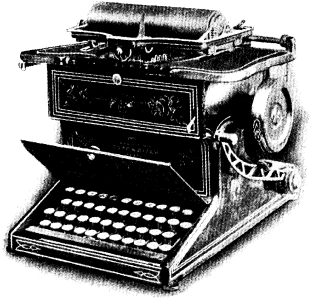
\includegraphics[width=\textwidth]{type_writer2.png}
\end{minipage}

\pause
\vfill

\textit{MRP 2019: Cross-Framework Meaning Representation Parsing} \citep{Oep:Abe:Haj:19}

\begin{itemize}
\item DM, PSD, EDS, UCCA and AMR parsing in English.
\end{itemize}

\pause
\vfill

\textit{MRP 2020: Cross-Framework and Cross-Lingual MRP} \citep{Oep:Abe:Abz:20}

\begin{itemize}
\item EDS, PTG, UCCA, AMR and DRG parsing in English, Czech, German and Chinese.
\end{itemize}
\end{frame}


\begin{frame}\frametitle{SemEval 2019 Task 1: Cross-lingual Semantic Parsing}
\begin{itemize}
\item UCCA parsing in English, French and German.
\item 8 teams participated.
\item Baseline: TUPA.
\end{itemize}

\vfill\pause

        \begin{itemize}
            \item 
                English $\{$in-domain/out-of-domain$\} \times 
                \{$open/closed$\}$
            \item
                German in-domain $\{$open/closed$\}$
            \item
                French \textit{low-resource} (only 15 training sentences)
        \end{itemize}

\vfill
\begin{center}
  \begin{minipage}{.2\textwidth}
\includegraphics[width=\textwidth]{wikipedia.png}\end{minipage}
  \begin{minipage}{.2\textwidth}
\includegraphics[width=\textwidth]{squid.jpg}\end{minipage}
\end{center}
\end{frame}

\begin{frame}
\frametitle{SemEval 2019 Task 1}
    \begin{figure}
        \centering
        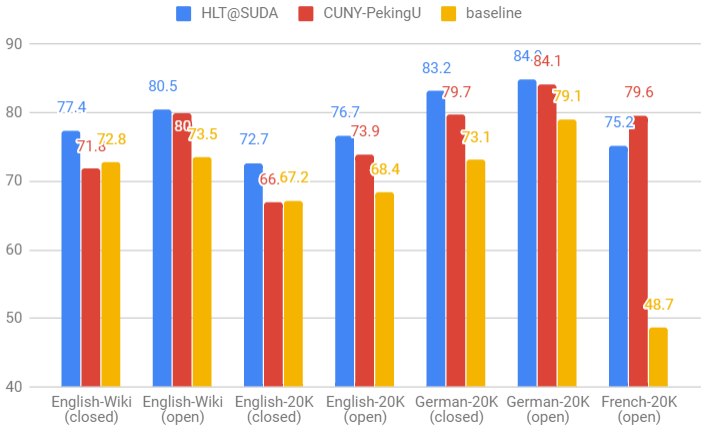
\includegraphics[width=\textwidth]{Capture}
    \end{figure}
\end{frame}

\begin{frame}
\frametitle{SemEval 2019 Task 1}

        HLT@SUDA: \\
        Neural constituency parser + multi-task + BERT \\
        French: trained on all languages, with language embedding
        
        \begin{center}
            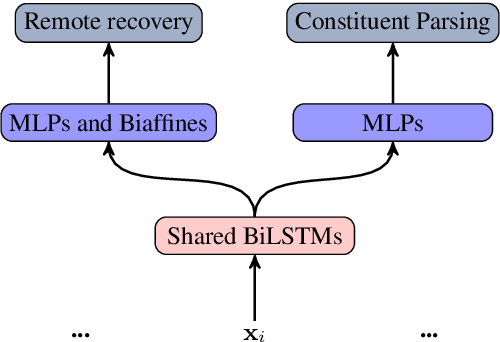
\includegraphics[width=.8\textwidth]{hltsuda3.png}
        \end{center}  
\end{frame}

\begin{frame}{MRP 2019}
\begin{itemize}
\item DM, PSD, EDS, UCCA and AMR parsing in English.
\item 18 teams participated.
\item Baseline: TUPA (generalized beyond UCCA).
\end{itemize}
\end{frame}



\pgfplotstableread{
a b c d e f shape	System	Approach	Overall	DM	PSD	EDS	UCCA	AMR
1 2 3 4 5 6 1	ERG	Composition	0.383	0.961	{}	0.952	{}	{}
1 2 3 4 5 6 3	{TUPA single}	Transition	0.577	0.555	0.518	0.810	0.276	0.447
1 2 3 4 5 6 3	{TUPA multi}	Transition	0.453	0.427	0.527	0.740	0.237	0.338
1 2 3 4 5 6 2	SJTU--NICT	Factorization	0.853	0.955	0.912	0.899	0.778	0.720
1 2 3 4 5 6 1	Saarland	Composition	0.819	0.947	0.913	0.891	0.676	0.667
1 2 3 4 5 6 3	{{\'U}FAL MRPipe}	Transition	0.747	0.849	0.763	0.675	0.732	0.718
1 2 3 4 5 6 3	{\'U}FAL--Oslo	Transition	0.344	0.805	0.609	0.306	{}	{}
1 2 3 4 5 6 2	Hitachi	Factorization	0.760	0.910	0.912	0.837	0.704	0.439
1 2 3 4 5 6 2	Amazon	Factorization	0.513	0.933	0.900	{}	{}	0.734
1 2 3 4 5 6 4	Bocharov	{}	0.065	{}	{}	{}	{}	0.327
1 2 3 4 5 6 3	HIT-SCIR	Transition	0.862	0.951	0.905	0.907	0.817	0.729
1 2 3 4 5 6 3	SJTU	Transition	0.430	0.432	0.476	0.532	0.327	0.385
1 2 3 4 5 6 2	SUDA--Alibaba	Factorization	0.840	0.923	0.856	0.918	0.784	0.717
1 2 3 4 5 6 2	JBNU	Factorization	0.465	0.940	0.879	{}	0.507	{}
1 2 3 4 5 6 4	HKUST	{}	0.245	0.370	0.353	{}	0.502	{}
1 2 3 4 5 6 2	ShanghaiTech	Factorization	0.670	0.949	0.895	0.869	{}	0.636
1 2 3 4 5 6 2	Peking	Factorization	0.711	0.944	0.894	0.945	0.772	{}
1 2 3 4 5 6 1	Peking	Composition	0.711	0.944	0.894	0.945	0.772	{}
1 2 3 4 5 6 4	Anonymous	{}	0.022	{}	0.109	{}	{}	{}
1 2 3 4 5 6 3	CUHK	Transition	0.378	0.687	0.648	0.276	0.196	0.081
}\approaches

\begin{frame}[fragile]
  \frametitle{Results}
  \begin{center}\footnotesize
\begin{tikzpicture}
    \begin{axis}[
    enlarge x limits={abs=7mm},
    ymin=.7,ymax=1,
    clip=true,
    ymajorgrids=true,
    width=\textwidth,
    height=.9\textheight,
    xtick={1,2,3,4,5,6},
    xticklabels={Overall,DM,PSD,EDS,UCCA,AMR},
    xticklabel style={font=\small,anchor=north},
    xtick align=inside,
    xticklabel pos=left,
    tickwidth=0pt,
    axis background/.style={fill=cyan!10},
    scatter/classes={1={mark=square,red,draw opacity=.5},
                   2={mark=triangle,black,draw opacity=.5},
                   3={mark=o,blue,draw opacity=.5},
                   4={mark=x,Purple,draw opacity=0}
                  },
    scatter,only marks,mark size=7,scatter src=explicit symbolic,
    legend style={font=\tiny}
    ]
    \addplot table[x=a,y=Overall,meta=shape]{\approaches};
    \addplot table[x=b,y=DM,meta=shape]{\approaches};
    \addplot table[x=c,y=PSD,meta=shape]{\approaches};
    \addplot table[x=d,y=EDS,meta=shape]{\approaches};
    \addplot table[x=e,y=UCCA,meta=shape]{\approaches};
    \addplot table[x=f,y=AMR,meta=shape]{\approaches};
    \legend{Composition,Factorization,Transition};
    \end{axis}
\end{tikzpicture}
  \end{center}
\end{frame}

\begin{frame}
\frametitle{MRP 2019}
Winning system: HIT-SCIR \citep{Che:Dou:Xu:19}.

Transition-based parser (similar to TUPA) + efficient training + BERT.

\begin{center}
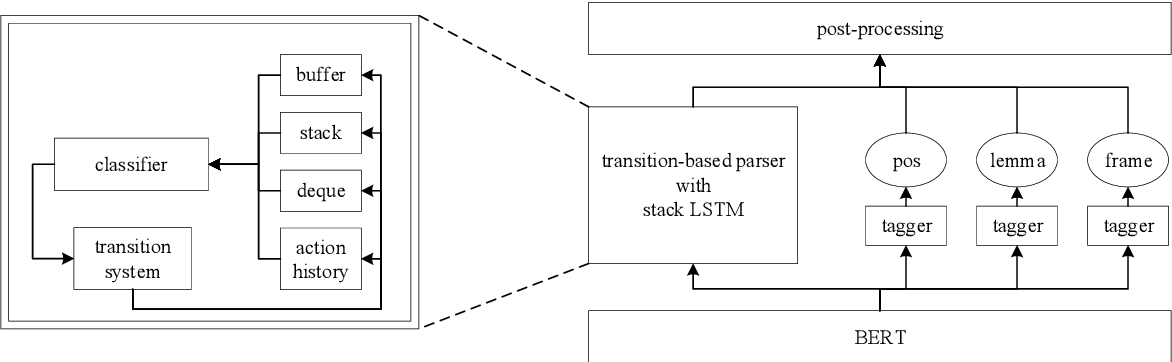
\includegraphics[width=\textwidth]{hitscir1}
\end{center}
\end{frame}

\begin{frame}{MRP 2020}
\begin{itemize}
\item EDS, PTG, UCCA, AMR and DRG parsing in English, Czech, German and Chinese.
\item 8 teams participated.
\end{itemize}
\end{frame}

\begin{frame}{MRP 2020}
\begin{center}
\begin{tabular}{lccccccccccccccc}
\toprule
 & \multicolumn{3}{c}{\textbf{EDS}} &  \multicolumn{3}{c}{\textbf{UCCA}} & \multicolumn{3}{c}{\textbf{AMR}} \\
\cmidrule(l{2pt}r{3pt}){2-4} \cmidrule(l{2pt}r{3pt}){5-7} \cmidrule(l{2pt}r{3pt}){8-10}
 & P & R & F & P & R & F & P & R & F\\
\midrule
2019 & .92 & .93 & .93 & .84 & .82 & .83 & .74 & .72 & .73 \\
2020 & .97 & .97 & .97 & .86 & .80 & .83 & .78 & .79 & .79 \\
\bottomrule
\end{tabular}
\end{center}
\end{frame}

\begin{frame}{MRP 2020}
Winning systems: \'{U}FAL \citep{Sam:Str:20} and Hitachi
    \citep{Oza:Mor:Kor:20}, encoder-decoder with pre-trained transformers.
\end{frame}


\pgfplotstableread{
framework {system} {eval f1} {best f1} {best name}
EDS {HIT-SCIR (Ours)} 80 94 Hitachi
PTG TUPA 54 89 Hitachi
UCCA TUPA 73 76 ÚFAL
AMR TUPA 52 82 Hitachi
DRG TUPA 63 94 ÚFAL
Overall All 64 86 {Hitachi \& ÚFAL}
}\cfscores

\frame{
\frametitle{Official Evaluation}
  Cross Framework Track:
  \vfill
  
    \begin{tikzpicture}
    \begin{axis}[
    ybar=0pt,
    enlarge x limits={abs=7mm},
    enlarge y limits={value=0.14,upper},
    ymin=0,
    clip=true,
    width=1.1\textwidth,
    height=.94\textheight,
    bar width=12pt,
    xtick=data,
    xticklabels from table={\cfscores}{framework},
    xticklabel style={font=\small,anchor=north},
    xtick align=inside,
    xticklabel pos=left,
    yticklabels=none,
    xlabel={\tiny Full Evaluation MRP F-score (\%)},
    tickwidth=0pt,
    nodes near coords={\scalebox{.6}{\pgfmathprintnumber[precision=1]{\pgfplotspointmeta}}},
    every node near coord/.append style={font=\small,rotate=90,anchor=west},
    axis background/.style={fill=cyan!10},
    legend style={at={(axis cs:5.4,0)},anchor=south east,font=\tiny},
    legend cell align={left},
    ]
    \addplot[fill=red]table[x expr=\coordindex,y=eval f1]{\cfscores};
    \addplot[fill=Gold]table[x expr=\coordindex,y=best f1]{\cfscores};
    \addplot+[color=black, point meta=explicit symbolic, only marks, nodes near coords, every node near coord/.append style={font=\tiny,anchor=east},xshift=-4mm]
    table[x expr=\coordindex,y=eval f1, meta=system, forget plot] {\cfscores};
    \addplot+[color=black, point meta=explicit symbolic, only marks, nodes near coords, every node near coord/.append style={font=\tiny,anchor=east}]
    table[x expr=\coordindex,y=best f1, meta=best name, forget plot] {\cfscores};
    \legend{Our System,Best System}
    \end{axis}
    \end{tikzpicture}
}

\pgfplotstableread{
framework {system} {eval f1} {best f1} {best name}
PTG TUPA 58 91 ÚFAL
UCCA {HIT-SCIR (Ous)} 75 81 ÚFAL
AMR TUPA 45 80 Hitachi
DRG TUPA 62 93 Hitachi
Overall All 60 85 {Hitachi \& ÚFAL}
}\clscores

\frame{
\frametitle{Official Evaluation}
  Cross Lingual Track:
  \vfill
  
    \begin{tikzpicture}
    \begin{axis}[
    ybar=0pt,
    enlarge x limits={abs=7mm},
    enlarge y limits={value=0.14,upper},
    ymin=0,
    clip=true,
    width=1.1\textwidth,
    height=.94\textheight,
    bar width=12pt,
    xtick=data,
    xticklabels from table={\clscores}{framework},
    xticklabel style={font=\small,anchor=north},
    xtick align=inside,
    xticklabel pos=left,
    yticklabels=none,
    xlabel={\tiny Full Evaluation MRP F-score (\%)},
    tickwidth=0pt,
    nodes near coords={\scalebox{.6}{\pgfmathprintnumber[precision=1]{\pgfplotspointmeta}}},
    every node near coord/.append style={font=\small,rotate=90,anchor=west},
    axis background/.style={fill=cyan!10},
    legend style={at={(axis cs:4.4,0)},anchor=south east,font=\tiny},
    legend cell align={left},
    ]
    \addplot[fill=red]table[x expr=\coordindex,y=eval f1]{\clscores};
    \addplot[fill=Gold]table[x expr=\coordindex,y=best f1]{\clscores};
    \addplot+[color=black, point meta=explicit symbolic, only marks, nodes near coords, every node near coord/.append style={font=\tiny,anchor=east},xshift=-4mm]
    table[x expr=\coordindex,y=eval f1, meta=system, forget plot] {\clscores};
    \addplot+[color=black, point meta=explicit symbolic, only marks, nodes near coords, every node near coord/.append style={font=\tiny,anchor=east}]
    table[x expr=\coordindex,y=best f1, meta=best name, forget plot] {\clscores};
    \legend{Our System,Best System}
    \end{axis}
    \end{tikzpicture}
}

\pgfplotstableread{
framework {system} {cf f1} {cl f1}
PTG TUPA 54 58
UCCA* HIT-SCIR 78 77
AMR TUPA 52 45
DRG* TUPA 52 51
}\cfvclscores

\pgfplotstableread{
framework {system} {cf data} {cl data}
PTG TUPA 42024 39560
UCCA  HIT-SCIR 6872 3713
AMR TUPA 16529 57885
DRG TUPA 6606 1575
}\cfvcldata

\frame{
\frametitle{CL vs. CF Track}
    \begin{tikzpicture}
    \begin{axis}[
    ybar=0pt,
    enlarge x limits={abs=7mm},
    enlarge y limits={value=0.34,upper},
    ymin=0,
    clip=true,
    width=1.1\textwidth,
    height=.45\textheight,
    bar width=12pt,
    xtick=data,
    xticklabels from table={\cfvclscores}{framework},
    xticklabel style={font=\small,anchor=north},
    xtick align=inside,
    xticklabel pos=left,
    yticklabels=none,
    xlabel={\tiny Full Evaluation (* for Validation) MRP F-score (\%)},
    tickwidth=0pt,
    nodes near coords={\scalebox{.6}{\pgfmathprintnumber[precision=1]{\pgfplotspointmeta}}},
    every node near coord/.append style={font=\small,rotate=90,anchor=west},
    axis background/.style={fill=cyan!10},
    legend style={at={(axis cs:3.2,80)},anchor=south east,font=\tiny},
    legend cell align={left},
    ]
    \addplot[fill=red]table[x expr=\coordindex,y=cf f1]{\cfvclscores};
    \addplot[fill=Gold]table[x expr=\coordindex,y=cl f1]{\cfvclscores};
    \addplot+[color=black, point meta=explicit symbolic, only marks, nodes near coords, every node near coord/.append style={font=\tiny,anchor=east},xshift=-4mm]
    table[x expr=\coordindex,y=cf f1, meta=system, forget plot] {\cfvclscores};
    \addplot+[color=black, point meta=explicit symbolic, only marks, nodes near coords, every node near coord/.append style={font=\tiny,anchor=east}]
    table[x expr=\coordindex,y=cl f1, meta=system, forget plot] {\cfvclscores};
    \legend{Cross-Framework,Cross-Lingual}
    \end{axis}
    \end{tikzpicture}
    
    \vfill
    
    \begin{tikzpicture}
    \begin{axis}[
    ybar=0pt,
    enlarge x limits={abs=7mm},
    enlarge y limits={value=0.8,upper},
    ymin=0,
    clip=true,
    width=1.1\textwidth,
    height=0.45\textheight,
    bar width=12pt,
    xtick=data,
    xticklabels from table={\cfvcldata}{framework},
    xticklabel style={font=\small,anchor=north},
    xtick align=inside,
    yticklabels=none,
    scaled y ticks=false,
    xlabel={\tiny Dataset Size (\# Sentences)},
    tickwidth=0pt,
    nodes near coords={\scalebox{.6}{\pgfmathprintnumber[precision=1]{\pgfplotspointmeta}}},
    every node near coord/.append style={font=\small,rotate=90,anchor=west},
    axis background/.style={fill=cyan!10},
    legend style={at={(axis cs:3.2,50000)},anchor=south east,font=\tiny},
    legend cell align={left},
    ]
    \addplot[fill=red]table[x expr=\coordindex,y=cf data]{\cfvcldata};
    \addplot[fill=Gold]table[x expr=\coordindex,y=cl data]{\cfvcldata};
    % \legend{Cross-Framework,Cross-Lingual}
    \end{axis}
    \end{tikzpicture}
}


\begin{frame}
	\frametitle{Multi-Task Model}
	{
	Variant 1
	  \begin{center}
	  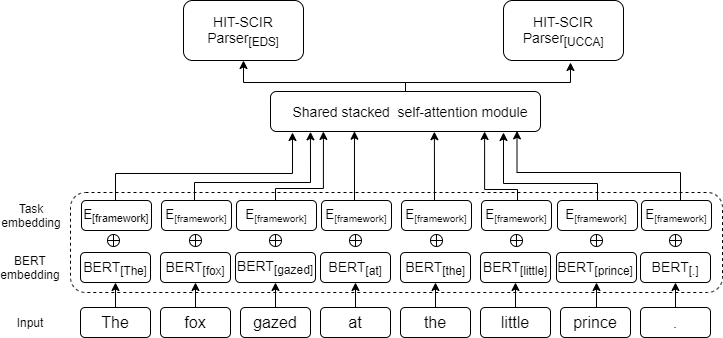
\includegraphics[width=.95\textwidth]{figures/multitask-shared.png}
	  \end{center}
	}
	\vspace{-1cm}
\end{frame}

\begin{frame}
	\frametitle{Multi-Task Model}
	{
	Variant 2
	  \begin{center}
	  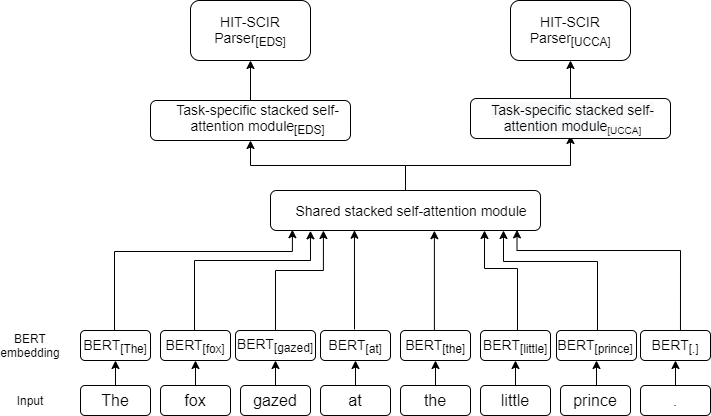
\includegraphics[width=.95\textwidth]{figures/multitask-dedicated.png}
	  \end{center}
	}
	\vspace{-1cm}
\end{frame}


\pgfplotstableread{
 framework Variant1 Variant2 Single-Task
 EDS 43 27 82
 UCCA 68 49 79
}\multitaskscores

\frame{
\frametitle{Multi-Task Results}
    \begin{tikzpicture}
    \begin{axis}[
    ybar=0pt,
    enlarge x limits={abs=23mm},
    enlarge y limits={value=0.14,upper},
    ymin=0,
    clip=true,
    width=1.1\textwidth,
    height=.94\textheight,
    bar width=28pt,
    xtick=data,
    xticklabels from table={\multitaskscores}{framework},
    xticklabel style={font=\small,anchor=north},
    xtick align=inside,
    xticklabel pos=left,
    yticklabels=none,
    xlabel={\tiny Cross-Framework Track Validation MRP F-score (\%)},
    tickwidth=0pt,
    nodes near coords={\scalebox{.6}{\pgfmathprintnumber[precision=1]{\pgfplotspointmeta}}},
    every node near coord/.append style={font=\small,rotate=90,anchor=west},
    axis background/.style={fill=cyan!10},
    legend style={at={(axis cs:1.4,0)},anchor=south east,font=\tiny},
    legend cell align={left},
    ]
    \addplot[fill=red]table[x expr=\coordindex,y=Variant1]{\multitaskscores};
    \addplot[fill=Gold]table[x expr=\coordindex,y=Variant2]{\multitaskscores};
    \addplot[fill=Green]table[x expr=\coordindex,y=Single-Task]{\multitaskscores};
    \legend{Variant 1,Variant 2,Single-Task}
    \end{axis}
    \end{tikzpicture}
}

\begin{frame}{IWPT 2020}
Applied HIT-SCIR parser to Enhanced UD parsing
\citep*{hershcovich-etal-2020-kopsala}.
\begin{center}
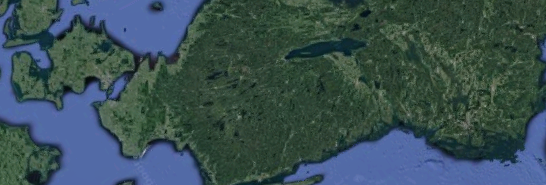
\includegraphics[width=.8\textwidth]{map_big}
\end{center}
\end{frame}


\begin{frame}{IWPT 2020}
  \begin{overlayarea}{\textwidth}{\textheight}
  \only<1-3>{
    \begin{block}{}
      \vspace{0.27cm}
    \end{block}{}
  }
  \only<4>{
    \begin{block}{}
      \centerline{\textcolor{lightgreen}{\textsc{Shift}}}
    \end{block}{}
  }
  \only<5>{
    \begin{block}{}
      \centerline{\textcolor{lightgreen}{\textsc{Shift}} x4}
    \end{block}{}
  }
  \only<6>{
    \begin{block}{}
      \centerline{\textcolor{lightgreen}{\textsc{Left-Edge:nmod}} }
    \end{block}{}
  }
  \only<7>{
    \begin{block}{}
      \centerline{\textcolor{lightgreen}{\textsc{Node}} }
    \end{block}{}
  }
  \only<8>{
    \begin{block}{}
      \centerline{\textcolor{lightgreen}{\textsc{Reduce-1}} }
    \end{block}{}
  }
  \only<9>{
    \begin{block}{}
      \centerline{\textcolor{lightgreen}{\textsc{Left-Edge:det}} }
    \end{block}{}
  }
  \only<10>{
    \begin{block}{}
      \centerline{\textcolor{lightgreen}{\textsc{Reduce-1}} }
    \end{block}{}
  }
  \only<11>{
    \begin{block}{}
      \vspace{0.12cm}
      \centerline{\ldots}
      \vspace{0.12cm}
    \end{block}{}
  }
  \only<12>{
    \begin{block}{}
      \centerline{\textcolor{lightgreen}{\textsc{Swap}} }
    \end{block}{}
  }
  \only<13>{
    \begin{block}{}
      \centerline{\textcolor{lightgreen}{\textsc{Right-Edge:nmod:van}} }
    \end{block}{}
  }
  \only<14>{
    \begin{block}{}
      \centerline{\textcolor{lightgreen}{\semitransp{\textsc{Reduce-0}} }}
    \end{block}{}
  }
  \only<15>{
    \begin{block}{}
      \centerline{\textcolor{lightgreen}{\semitransp{\textsc{Shift}} x3} }
    \end{block}{}
  }
  \only<16>{
    \begin{block}{}
      \centerline{\textcolor{lightgreen}{\textsc{Swap}} }
    \end{block}{}
  }
  \only<17>{
    \begin{block}{}
      \centerline{\textcolor{lightgreen}{\semitransp{\textsc{Right-Edge:cc}}} }
    \end{block}{}
  }
  \only<18>{
    \begin{block}{}
      \centerline{\textcolor{lightgreen}{\semitransp{\textsc{Reduce-0}}} }
    \end{block}{}
  }
  \only<19>{
    \begin{block}{}
      \centerline{\textcolor{lightgreen}{\semitransp{\textsc{Shift}} x2} }
    \end{block}{}
  }
  \only<20>{
    \begin{block}{}
      \centerline{\textcolor{lightgreen}{\textsc{Swap}} }
    \end{block}{}
  }
  \only<21>{
    \begin{block}{}
      \vspace{0.12cm}
      \centerline{\ldots}
      \vspace{0.12cm}
    \end{block}{}
  }
  \only<22>{
    \begin{block}{}
      \centerline{\textcolor{lightgreen}{\semitransp{\textsc{Right-Edge:punct}}} }
    \end{block}{}
  }
  \only<23>{
    \begin{block}{}
      \centerline{\textcolor{lightgreen}{\semitransp{\textsc{Reduce-0}} x2} }
    \end{block}{}
  }
  \only<24>{
    \begin{block}{}
      \centerline{\textcolor{lightgreen}{\textsc{Finish}} }
    \end{block}{}
  }

\only<1-5>{
  \begin{figure}[ht]
    \centering
    \begin{dependency}[text only label, label style={above}, font=\tiny, scale=0.5]
      \begin{deptext}[column sep=0em]
        Deze \& is  \& de  \& grootste \& hal  \& van \& België \& , \& en  \& \textit{NULL}  \& de  \& enige \& die  \& voldoet \& aan \& de  \& normen \& .     \\
      \end{deptext}
      \depedge{5}{1}{nsubj}
      \depedge{5}{2}{cop}
      \depedge{5}{3}{det}
      \depedge[edge below]{5}{4}{nmod}
      \deproot[edge unit distance=2ex]{5}{root}
      \depedge{7}{6}{case}
      \depedge{5}{7}{nmod\textbf{:van}}
      \depedge[edge unit distance=.8ex]{12}{8}{punct}
    %   \depedge[dashed]{12}{9}{cc}
      \depedge[edge below]{10}{9}{cc}
      \depedge[edge below]{5}{10}{conj:en}
      \depedge[edge unit distance=2ex]{14}{10}{nsubj:relsubj}
    %   \depedge[dashed]{12}{11}{det}
      \depedge[edge below]{10}{11}{det}
    %   \depedge[dashed,edge unit distance=1ex]{5}{12}{conj}
      \depedge[edge below]{10}{12}{nmod}
    %   \depedge[dashed]{14}{13}{nsubj}
      \depedge[edge below]{10}{13}{ref}
    %   \depedge[dashed]{12}{14}{acl:relcl}
      \depedge[edge below,edge unit distance=4.7ex]{10}{14}{acl:relcl}
      \depedge{17}{15}{case}
      \depedge{17}{16}{det}
      \depedge{14}{17}{obl\textbf{:aan}}
      \depedge[edge unit distance=1.2ex]{5}{18}{punct}
    \end{dependency}
  \end{figure}
}

  \only<6-8>{
  \begin{figure}[ht]
    \centering
    \begin{dependency}[text only label, label style={above}, font=\tiny, scale=0.5]
      \begin{deptext}[column sep=0em]
        Deze \& is  \& de  \& grootste \& hal  \& van \& België \& , \& en  \& \textit{NULL}  \& de  \& enige \& die  \& voldoet \& aan \& de  \& normen \& .     \\
      \end{deptext}
      \depedge{5}{1}{nsubj}
      \depedge{5}{2}{cop}
      \depedge{5}{3}{det}
      \depedge[green,edge below]{5}{4}{nmod}
      \deproot[edge unit distance=2ex]{5}{root}
      \depedge{7}{6}{case}
      \depedge{5}{7}{nmod\textbf{:van}}
      \depedge[edge unit distance=.8ex]{12}{8}{punct}
    %   \depedge[dashed]{12}{9}{cc}
      \depedge[edge below]{10}{9}{cc}
      \depedge[edge below]{5}{10}{conj:en}
      \depedge[edge unit distance=2ex]{14}{10}{nsubj:relsubj}
    %   \depedge[dashed]{12}{11}{det}
      \depedge[edge below]{10}{11}{det}
    %   \depedge[dashed,edge unit distance=1ex]{5}{12}{conj}
      \depedge[edge below]{10}{12}{nmod}
    %   \depedge[dashed]{14}{13}{nsubj}
      \depedge[edge below]{10}{13}{ref}
    %   \depedge[dashed]{12}{14}{acl:relcl}
      \depedge[edge below,edge unit distance=4.7ex]{10}{14}{acl:relcl}
      \depedge{17}{15}{case}
      \depedge{17}{16}{det}
      \depedge{14}{17}{obl\textbf{:aan}}
      \depedge[edge unit distance=1.2ex]{5}{18}{punct}
    \end{dependency}
\end{figure}
}

\only<9-10>{
  \begin{figure}[ht]
    \centering
    \begin{dependency}[text only label, label style={above}, font=\tiny, scale=0.5]
      \begin{deptext}[column sep=0em]
        Deze \& is  \& de  \& grootste \& hal  \& van \& België \& , \& en  \& \textit{NULL}  \& de  \& enige \& die  \& voldoet \& aan \& de  \& normen \& .     \\
      \end{deptext}
      \depedge{5}{1}{nsubj}
      \depedge{5}{2}{cop}
      \depedge[green]{5}{3}{det}
      \depedge[green,edge below]{5}{4}{nmod}
      \deproot[edge unit distance=2ex]{5}{root}
      \depedge{7}{6}{case}
      \depedge{5}{7}{nmod\textbf{:van}}
      \depedge[edge unit distance=.8ex]{12}{8}{punct}
    %   \depedge[dashed]{12}{9}{cc}
      \depedge[edge below]{10}{9}{cc}
      \depedge[edge below]{5}{10}{conj:en}
      \depedge[edge unit distance=2ex]{14}{10}{nsubj:relsubj}
    %   \depedge[dashed]{12}{11}{det}
      \depedge[edge below]{10}{11}{det}
    %   \depedge[dashed,edge unit distance=1ex]{5}{12}{conj}
      \depedge[edge below]{10}{12}{nmod}
    %   \depedge[dashed]{14}{13}{nsubj}
      \depedge[edge below]{10}{13}{ref}
    %   \depedge[dashed]{12}{14}{acl:relcl}
      \depedge[edge below,edge unit distance=4.7ex]{10}{14}{acl:relcl}
      \depedge{17}{15}{case}
      \depedge{17}{16}{det}
      \depedge{14}{17}{obl\textbf{:aan}}
      \depedge[edge unit distance=1.2ex]{5}{18}{punct}
    \end{dependency}
  \end{figure}
}


\only<11-12>{
  \begin{figure}[ht]
    \centering
    \begin{dependency}[text only label, label style={above}, font=\tiny, scale=0.5]
      \begin{deptext}[column sep=0em]
        Deze \& is  \& de  \& grootste \& hal  \& van \& België \& , \& en  \& \textit{NULL}  \& de  \& enige \& die  \& voldoet \& aan \& de  \& normen \& .     \\
      \end{deptext}
      \depedge[green]{5}{1}{nsubj}
      \depedge[green]{5}{2}{cop}
      \depedge[green]{5}{3}{det}
      \depedge[green,edge below]{5}{4}{nmod}
      \deproot[green,edge unit distance=2ex]{5}{root}
      \depedge[green]{7}{6}{case}
      \depedge{5}{7}{nmod\textbf{:van}}
      \depedge[edge unit distance=.8ex]{12}{8}{punct}
    %   \depedge[dashed]{12}{9}{cc}
      \depedge[edge below]{10}{9}{cc}
      \depedge[green,edge below]{5}{10}{conj:en}
      \depedge[edge unit distance=2ex]{14}{10}{nsubj:relsubj}
    %   \depedge[dashed]{12}{11}{det}
      \depedge[edge below]{10}{11}{det}
    %   \depedge[dashed,edge unit distance=1ex]{5}{12}{conj}
      \depedge[edge below]{10}{12}{nmod}
    %   \depedge[dashed]{14}{13}{nsubj}
      \depedge[edge below]{10}{13}{ref}
    %   \depedge[dashed]{12}{14}{acl:relcl}
      \depedge[edge below,edge unit distance=4.7ex]{10}{14}{acl:relcl}
      \depedge{17}{15}{case}
      \depedge{17}{16}{det}
      \depedge{14}{17}{obl\textbf{:aan}}
      \depedge[edge unit distance=1.2ex]{5}{18}{punct}
    \end{dependency}
  \end{figure}
}

\only<13-16>{
  \begin{figure}[ht]
    \centering
    \begin{dependency}[text only label, label style={above}, font=\tiny, scale=0.5]
      \begin{deptext}[column sep=0em]
        Deze \& is  \& de  \& grootste \& hal  \& van \& België \& , \& en  \& \textit{NULL}  \& de  \& enige \& die  \& voldoet \& aan \& de  \& normen \& .     \\
      \end{deptext}
      \depedge[green]{5}{1}{nsubj}
      \depedge[green]{5}{2}{cop}
      \depedge[green]{5}{3}{det}
      \depedge[green,edge below]{5}{4}{nmod}
      \deproot[green,edge unit distance=2ex]{5}{root}
      \depedge[green]{7}{6}{case}
      \depedge[green]{5}{7}{nmod\textbf{:van}}
      \depedge[edge unit distance=.8ex]{12}{8}{punct}
    %   \depedge[dashed]{12}{9}{cc}
      \depedge[edge below]{10}{9}{cc}
      \depedge[green,edge below]{5}{10}{conj:en}
      \depedge[edge unit distance=2ex]{14}{10}{nsubj:relsubj}
    %   \depedge[dashed]{12}{11}{det}
      \depedge[edge below]{10}{11}{det}
    %   \depedge[dashed,edge unit distance=1ex]{5}{12}{conj}
      \depedge[edge below]{10}{12}{nmod}
    %   \depedge[dashed]{14}{13}{nsubj}
      \depedge[edge below]{10}{13}{ref}
    %   \depedge[dashed]{12}{14}{acl:relcl}
      \depedge[edge below,edge unit distance=4.7ex]{10}{14}{acl:relcl}
      \depedge{17}{15}{case}
      \depedge{17}{16}{det}
      \depedge{14}{17}{obl\textbf{:aan}}
      \depedge[edge unit distance=1.2ex]{5}{18}{punct}
    \end{dependency}
  \end{figure}
}

\only<17-20>{
  \begin{figure}[ht]
    \centering
    \begin{dependency}[text only label, label style={above}, font=\tiny, scale=0.5]
      \begin{deptext}[column sep=0em]
        Deze \& is  \& de  \& grootste \& hal  \& van \& België \& , \& en  \& \textit{NULL}  \& de  \& enige \& die  \& voldoet \& aan \& de  \& normen \& .     \\
      \end{deptext}
      \depedge[green]{5}{1}{nsubj}
      \depedge[green]{5}{2}{cop}
      \depedge[green]{5}{3}{det}
      \depedge[green,edge below]{5}{4}{nmod}
      \deproot[green,edge unit distance=2ex]{5}{root}
      \depedge[green]{7}{6}{case}
      \depedge[green]{5}{7}{nmod\textbf{:van}}
      \depedge[edge unit distance=.8ex]{12}{8}{punct}
    %   \depedge[dashed]{12}{9}{cc}
      \depedge[green,edge below]{10}{9}{cc}
      \depedge[green,edge below]{5}{10}{conj:en}
      \depedge[edge unit distance=2ex]{14}{10}{nsubj:relsubj}
    %   \depedge[dashed]{12}{11}{det}
      \depedge[edge below]{10}{11}{det}
    %   \depedge[dashed,edge unit distance=1ex]{5}{12}{conj}
      \depedge[edge below]{10}{12}{nmod}
    %   \depedge[dashed]{14}{13}{nsubj}
      \depedge[edge below]{10}{13}{ref}
    %   \depedge[dashed]{12}{14}{acl:relcl}
      \depedge[edge below,edge unit distance=4.7ex]{10}{14}{acl:relcl}
      \depedge{17}{15}{case}
      \depedge{17}{16}{det}
      \depedge{14}{17}{obl\textbf{:aan}}
      \depedge[edge unit distance=1.2ex]{5}{18}{punct}
    \end{dependency}
  \end{figure}
}

\only<21>{
  \begin{figure}[ht]
    \centering
    \begin{dependency}[text only label, label style={above}, font=\tiny, scale=0.5]
      \begin{deptext}[column sep=0em]
        Deze \& is  \& de  \& grootste \& hal  \& van \& België \& , \& en  \& \textit{NULL}  \& de  \& enige \& die  \& voldoet \& aan \& de  \& normen \& .     \\
      \end{deptext}
      \depedge[green]{5}{1}{nsubj}
      \depedge[green]{5}{2}{cop}
      \depedge[green]{5}{3}{det}
      \depedge[green,edge below]{5}{4}{nmod}
      \deproot[green,edge unit distance=2ex]{5}{root}
      \depedge[green]{7}{6}{case}
      \depedge[green]{5}{7}{nmod\textbf{:van}}
      \depedge[green,edge unit distance=.8ex]{12}{8}{punct}
    %   \depedge[green,dashed]{12}{9}{cc}
      \depedge[green,edge below]{10}{9}{cc}
      \depedge[green,edge below]{5}{10}{conj:en}
      \depedge[green,edge unit distance=2ex]{14}{10}{nsubj:relsubj}
    %   \depedge[green,dashed]{12}{11}{det}
      \depedge[green,edge below]{10}{11}{det}
    %   \depedge[green,dashed,edge unit distance=1ex]{5}{12}{conj}
      \depedge[green,edge below]{10}{12}{nmod}
    %   \depedge[green,dashed]{14}{13}{nsubj}
      \depedge[green,edge below]{10}{13}{ref}
    %   \depedge[green,dashed]{12}{14}{acl:relcl}
      \depedge[green,edge below,edge unit distance=4.7ex]{10}{14}{acl:relcl}
      \depedge[green]{17}{15}{case}
      \depedge[green]{17}{16}{det}
      \depedge[green]{14}{17}{obl\textbf{:aan}}
      \depedge[edge unit distance=1.2ex]{5}{18}{punct}
    \end{dependency}
  \end{figure}
}


\only<22->{
  \begin{figure}[ht]
    \centering
    \begin{dependency}[text only label, label style={above}, font=\tiny, scale=0.5]
      \begin{deptext}[column sep=0em]
        Deze \& is  \& de  \& grootste \& hal  \& van \& België \& , \& en  \& \textit{NULL}  \& de  \& enige \& die  \& voldoet \& aan \& de  \& normen \& .     \\
      \end{deptext}
      \depedge[green]{5}{1}{nsubj}
      \depedge[green]{5}{2}{cop}
      \depedge[green]{5}{3}{det}
      \depedge[green,edge below]{5}{4}{nmod}
      \deproot[green,edge unit distance=2ex]{5}{root}
      \depedge[green]{7}{6}{case}
      \depedge[green]{5}{7}{nmod\textbf{:van}}
      \depedge[green,edge unit distance=.8ex]{12}{8}{punct}
    %   \depedge[green,dashed]{12}{9}{cc}
      \depedge[green,edge below]{10}{9}{cc}
      \depedge[green,edge below]{5}{10}{conj:en}
      \depedge[green,edge unit distance=2ex]{14}{10}{nsubj:relsubj}
    %   \depedge[green,dashed]{12}{11}{det}
      \depedge[green,edge below]{10}{11}{det}
    %   \depedge[green,dashed,edge unit distance=1ex]{5}{12}{conj}
      \depedge[green,edge below]{10}{12}{nmod}
    %   \depedge[green,dashed]{14}{13}{nsubj}
      \depedge[green,edge below]{10}{13}{ref}
    %   \depedge[green,dashed]{12}{14}{acl:relcl}
      \depedge[green,edge below,edge unit distance=4.7ex]{10}{14}{acl:relcl}
      \depedge[green]{17}{15}{case}
      \depedge[green]{17}{16}{det}
      \depedge[green]{14}{17}{obl\textbf{:aan}}
      \depedge[green,edge unit distance=1.2ex]{5}{18}{punct}
    \end{dependency}
  \end{figure}
}


\only<1>{
  \begin{block}{}
    \vspace{0.39cm}
  \end{block}
}

\only<2>{
  \begin{block}{}
    $[$ ROOT $]$ $[$ \tiny{Deze is de grootste hal van België , en de enige die voldoet aan de normen .} $]$ 
  \end{block}
}
\only<3>{
  \begin{block}{}
    $[$ ROOT $]$ $[$ Deze is de grootste hal van België , en de (\dots) $]$ 
  \end{block}
}
\only<4>{
  \begin{block}{}
    $[$ ROOT Deze $]$ $[$ is de grootste hal van België , en de (\dots) $]$ 
  \end{block}
}
\only<5-6>{
  \begin{block}{}
    $[$ ROOT Deze is de grootste hal $]$ $[$ van België , en de (\dots) $]$ 
  \end{block}
}
\only<7>{
  \begin{block}{}
    $[$ ROOT Deze is de grootste hal $]$ $[$ NULL van België , en (\dots) $]$ 
  \end{block}
}
\only<8-9>{
  \begin{block}{}
    $[$ ROOT Deze is de hal $]$ $[$ NULL van België , en de enige (\dots) $]$ 
  \end{block}
}
\only<10>{
  \begin{block}{}
    $[$ ROOT Deze is hal $]$ $[$ NULL van België , en de enige die (\dots) $]$ 
  \end{block}
}
\only<11>{
  \begin{block}{}
    $[$ ROOT hal NULL België $]$ $[$ , en de enige die voldoet aan (\ldots) $]$ 
  \end{block}
}

\only<12-13>{
  \begin{block}{}
    $[$  ROOT hal België $]$ $[$ NULL , en de enige die voldoet aan (\dots) $]$ 
  \end{block}
}
\only<14>{
  \begin{block}{}
    $[$  ROOT hal $]$ $[$ NULL , en de enige die voldoet aan de normen $]$ 
  \end{block}
}
\only<15>{
  \begin{block}{}
    $[$  ROOT hal NULL , en $]$ $[$ de enige die voldoet aan de normen $]$ 
  \end{block}
}
\only<16-17>{
  \begin{block}{}
    $[$ ROOT hal NULL en $]$ $[$ , de enige die voldoet aan de normen $]$ 
  \end{block}
}
\only<18>{
  \begin{block}{}
    $[$   ROOT hal NULL $]$ $[$ , de enige die voldoet aan de normen $]$ 
  \end{block}
}
\only<19>{
  \begin{block}{}
    $[$  ROOT hal NULL , de $]$ $[$ enige die voldoet aan de normen $]$ 
  \end{block}
}
\only<20>{
  \begin{block}{}
    $[$  ROOT hal NULL de $]$ $[$ , enige die voldoet aan de normen $]$ 
  \end{block}
}
\only<21-22>{
  \begin{block}{}
    $[$  ROOT hal . $]$ $[$  $]$ 
  \end{block}
}
\only<23->{
  \begin{block}{}
    $[$  ROOT $]$ $[$  $]$ 
  \end{block}
}

\end{overlayarea}
\end{frame}

\section{Applications}

\begin{frame}
\frametitle{What can meaning representation do for NLP?}
 \begin{itemize}
 \item Incorporating linguistically informed rules
 \item Controlled evaluation by explicit criteria
 \item Inductive bias to facilitate learning
 \item Explainable models by design
 \end{itemize}
\end{frame}

\subsection{Incorporating linguistically informed rules into NLP}

\begin{frame}
\frametitle{Sentence Splitting for Text Simplification}
% https://www.aclweb.org/anthology/attachments/P18-1016.Presentation.pdf
    
    {\color{blue}Last year I read the book John authored} $\rightarrow$ \\
    \hfill {\color{red}John wrote a book.} {\color{green}I read the book.}
    
    \vfill\pause

    MT-based simplifcation is \textit{overly conservative}.
    
    \vfill\pause
    
    \textbf{Direct Semantic Splitting} before MT-based simplification
    to place each scene in its own sentence
    \citep{sulem-etal-2018-simple}.
    
    \begin{center}
        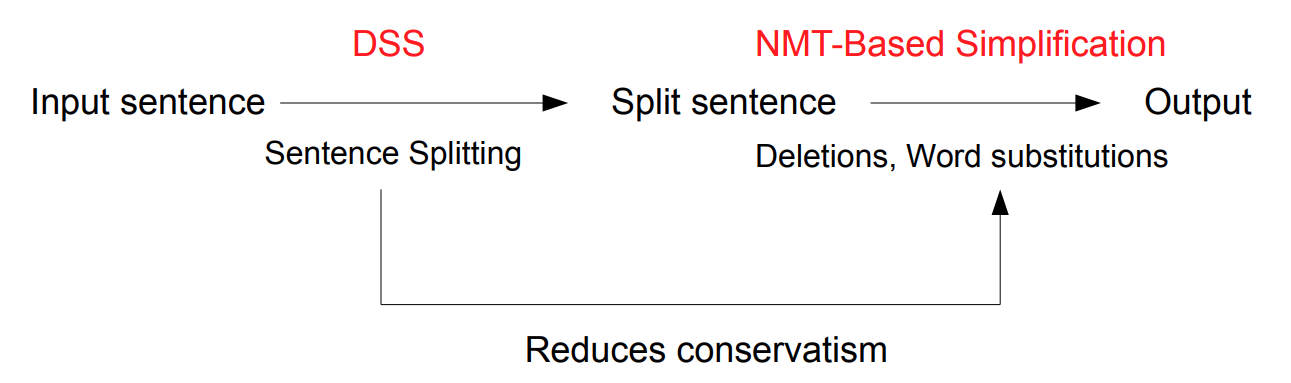
\includegraphics[width=.7\textwidth]{dss1.png}
    \end{center}
\end{frame}

\begin{frame}
\frametitle{Sentence Splitting for Text Simplification}
    \begin{center}
        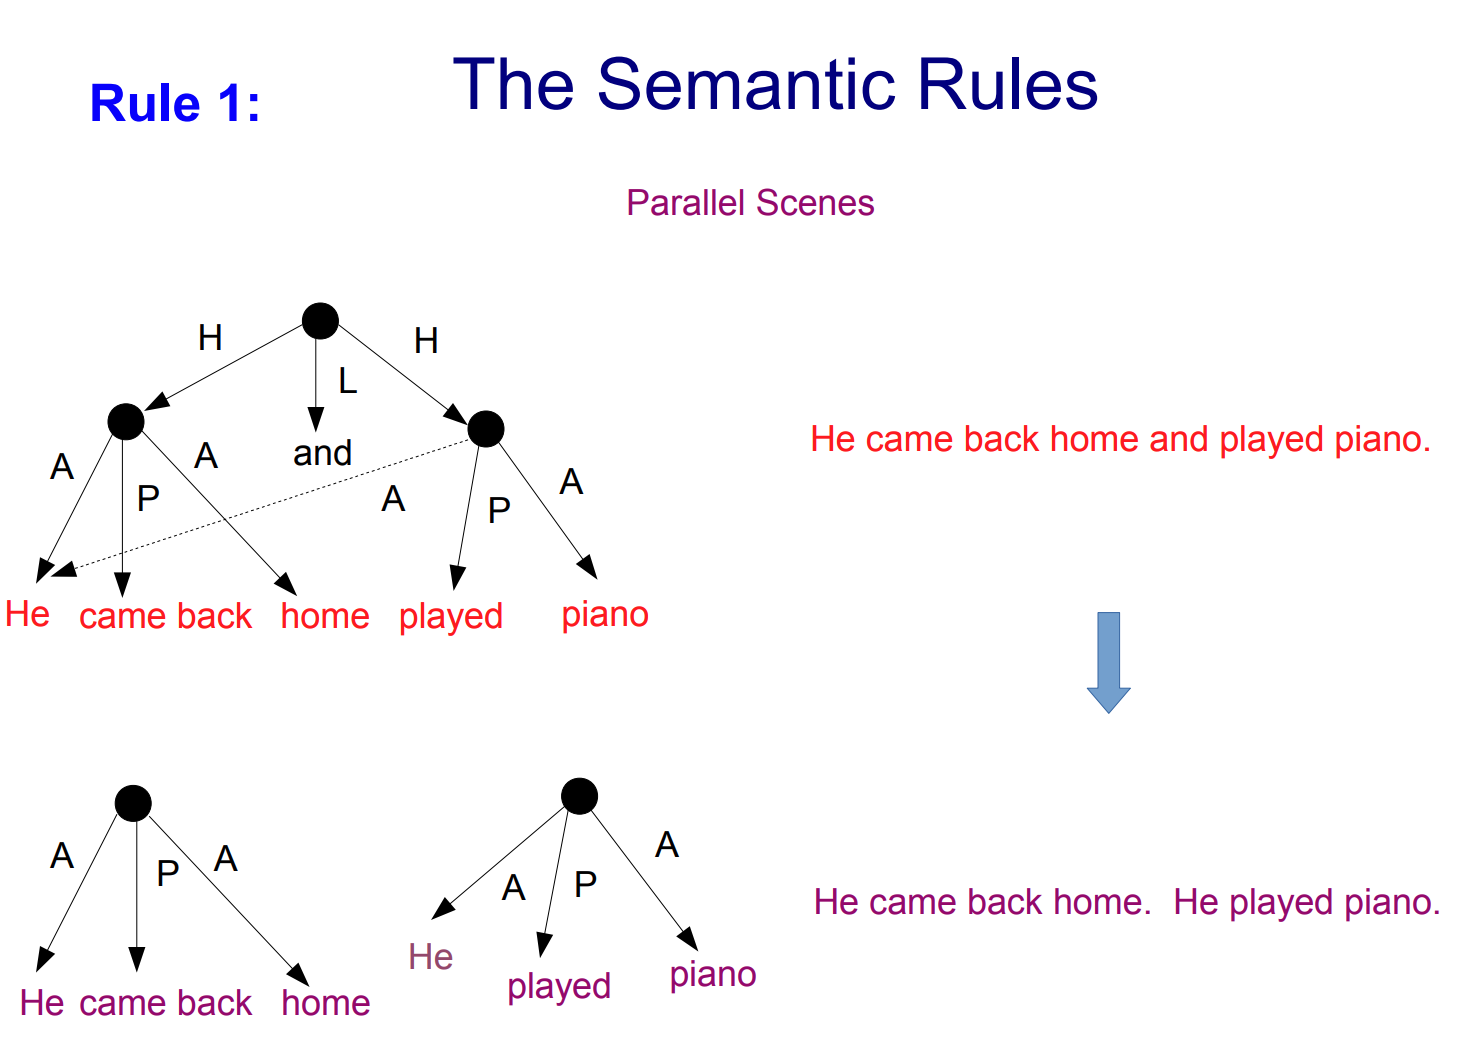
\includegraphics[width=\textwidth]{dss2.png}
    \end{center}
\end{frame}

\begin{frame}
\frametitle{Sentence Splitting for Text Simplification}
    \begin{center}
        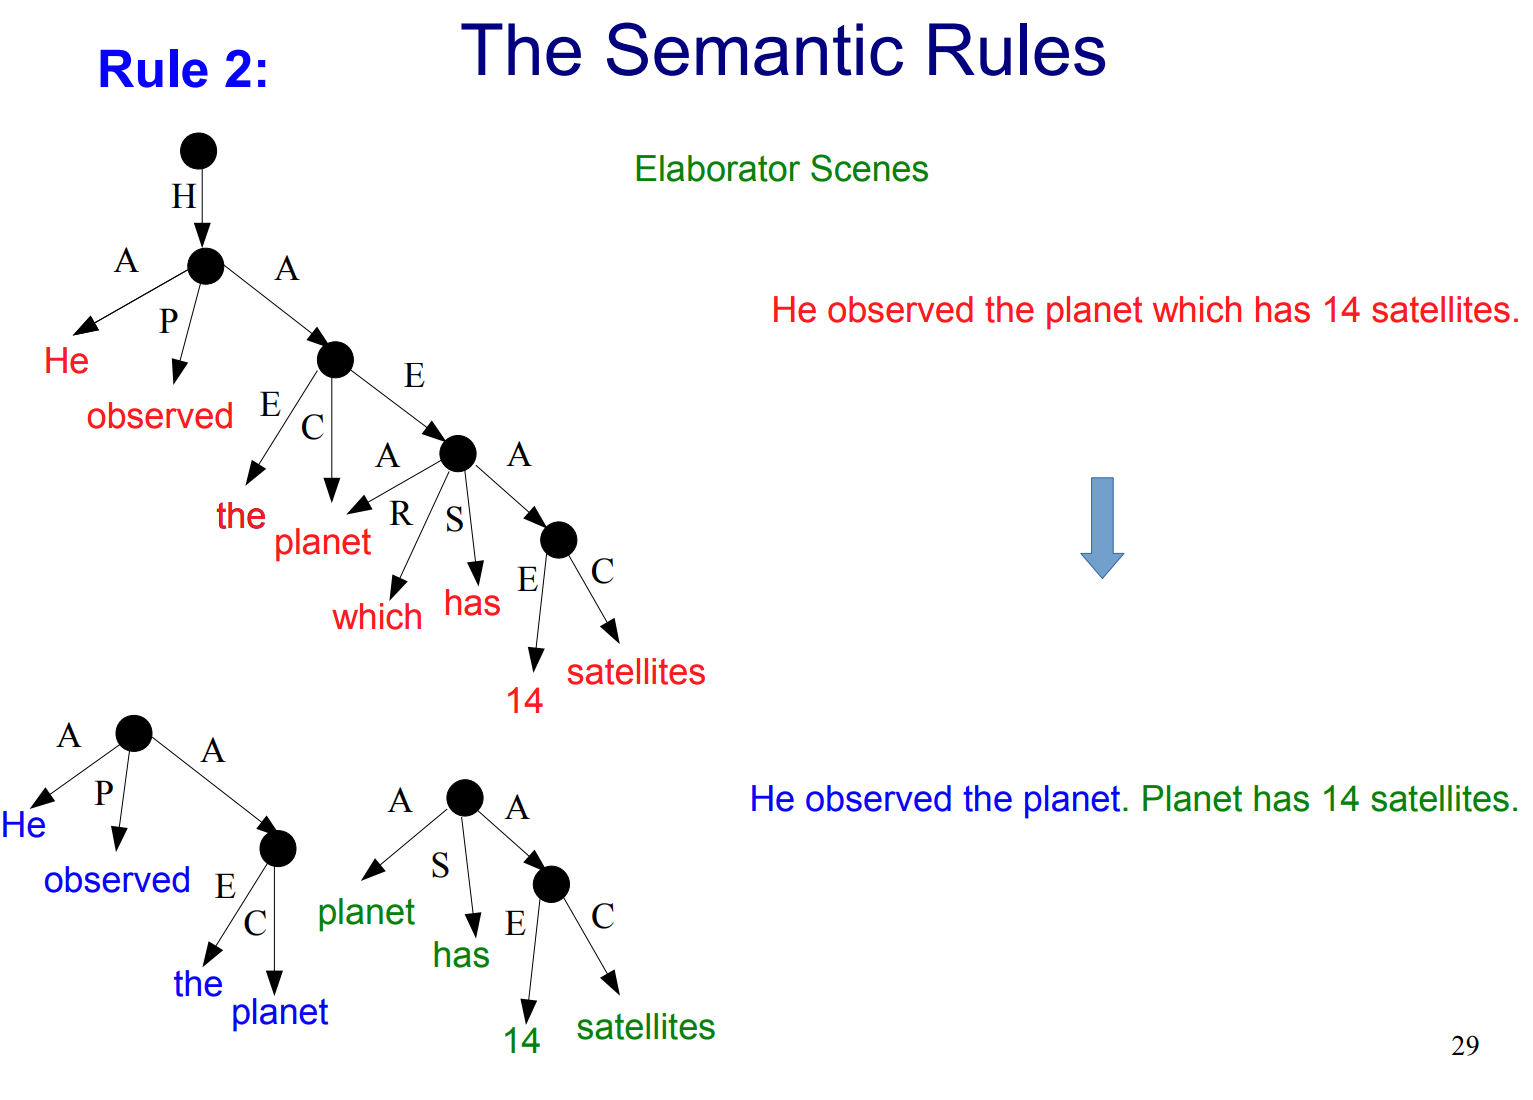
\includegraphics[width=\textwidth]{dss3.png}
    \end{center}
\end{frame}

\begin{frame}
\frametitle{Sentence Splitting for Text Simplification}
    Participant scenes are not split.
    \begin{center}
        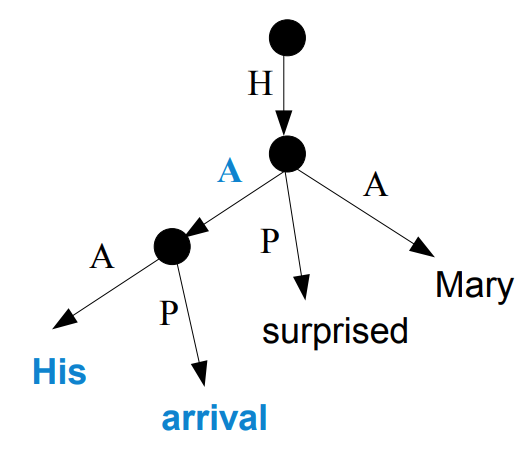
\includegraphics[width=.5\textwidth]{dss4.png}
    \end{center}
\end{frame}

\begin{frame}
\frametitle{Sentence Splitting for Text Simplification}
    {\color{blue}He observed the planet.} {\color{green}Planet has 14 satellites.}

    \vfill\pause
    
    Neural MT methods to fix grammaticality.
    \begin{center}
        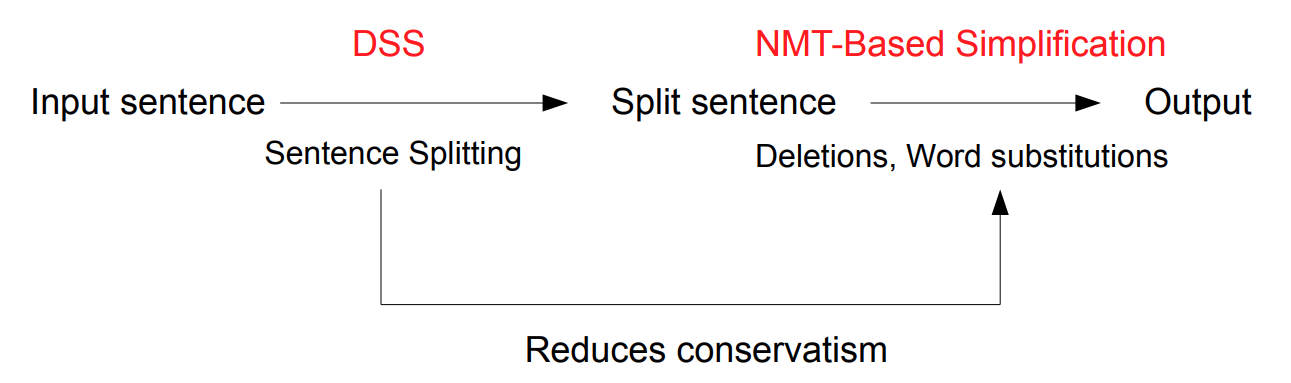
\includegraphics[width=\textwidth]{dss1.png}
    \end{center}
    
    \vfill\pause
    
    {\color{blue}He observed the planet.} {\color{green}\textbf{The planet} has 14 satellites.}
\end{frame}

% \begin{frame}
% \frametitle{Semantic Structural Decomposition for Neural Machine Translation}
%     \citep{sulem-etal-2020-semantic}.
% \end{frame}

\subsection{Controlled NLG evaluation by explicit criteria}

\begin{frame}{BLEU is Not Suitable for the Evaluation of Text Simplification}
    \textbf{BLEU}: reference-based evaluation metric for MT,
    also widely used to evaluate text simplification.
    
    \vfill\pause
    
    With sentence splitting,
    not correlated with grammaticality or meaning preservation
    \citep{sulem-etal-2018-bleu}.
    
    \vfill\pause
    
    \textit{Negatively correlated} with simplicity!
\end{frame}

\begin{frame}{Semantic Structural Evaluation for Text Simplification}
    \textbf{SAMSA}: reference-less measure of
    \textit{structural simplicity} and \textit{meaning preservation}
     \citep{sulem-etal-2018-semantic}.
     
    Same principle: \textit{one scene per sentence}.
    
    \begin{center}
        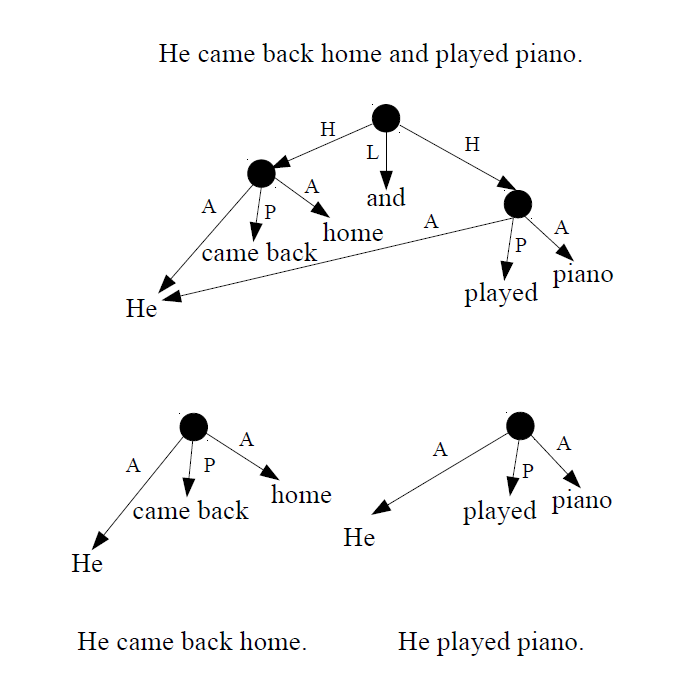
\includegraphics[width=.5\textwidth]{ucca_simplification}
    \end{center}
\end{frame}

\begin{frame}{Semantic Structural Evaluation for Text Simplification}
    \begin{center}
        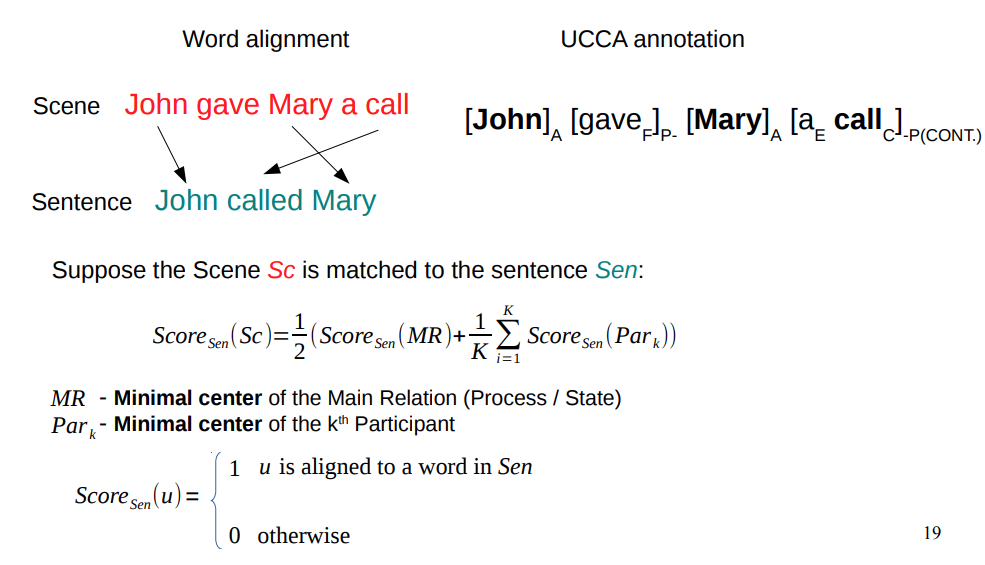
\includegraphics[width=.8\textwidth]{samsa1.png}
    \end{center}
    \begin{center}
        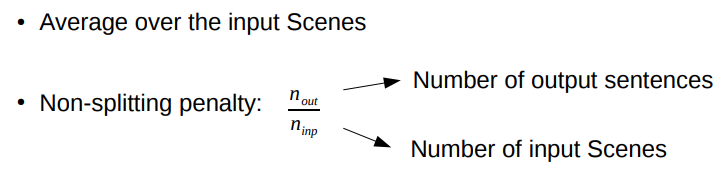
\includegraphics[width=.7\textwidth]{samsa2.png}
    \end{center}
\end{frame}

\begin{frame}{Grammatical Error Correction}
    Another text-to-text generation task.
    
    {\color{red}Ther is both sides of stories} \rightarrow \\
    \hfill {\color{blue}There are two sides to every story}
    
    \vfill\pause
    
    Using \textit{references} for GEC evaluation encourages conservatism and underestimates precision
    \citep{choshen-abend-2018-inherent}.
\end{frame}

\begin{frame}{Reference-less Measure of Faithfulness for Grammatical Error Correction}
    \begin{itemize}
        \item UCCA is \textit{applicable} to ungrammatical learner language!
        \item UCCA is \textit{stable} with respect to grammar corrections
    \end{itemize}
    
    \begin{center}
    \begin{tikzpicture}[sibling distance=3mm, level distance=7mm,
    every node/.append style={font=\rmfamily},
	every circle node/.append style={fill=black}]
    \begin{scope}[frontier/.style={distance from root=15mm},
	edge from parent path={(\tikzparentnode.center) ..
        controls +(0,-.25) and +(0,.25) .. (\tikzchildnode.north)}]
    \Tree [.\node [circle] (rootu) {};
    \edge node [auto=right]{}; \node (Heu) {He};
    \edge node[auto=right down]{}; \node (gve) {gve};
    \edge node[auto=right]{};
    [.\node [circle](an appleu) {};
    \edge node[auto=right]{}; \node (anu) {an};
    \edge node[auto=left]{}; \node (appleu) {apple};
    ]
    \edge node[auto=left]{};
    [.\node [circle](for john) {};
    \edge node[auto=right]{};\node (for) {for};
    \edge node[auto=left]{}; \node (john) {john};
    ]]
    \end{scope}
    \begin{scope}[yshift=-41mm,grow'=up,
      frontier/.style={distance from root=12mm},
      edge from parent path={(\tikzparentnode.center) ..
      controls +(0,.25) and +(0,-.25) .. (\tikzchildnode.south)}]
    \Tree [.\node [circle] (rootd) {};
    \edge node [auto=left]{}; \node (Hed) {He};
    \edge node[auto=right]{}; \node (gave) {gave};
    \edge node[auto=right]{};\node (John) {John};
    \edge node[auto=right]{};
    [.\node [circle] (an appled) {};
    \edge node[auto=left]{}; \node (and) {an};
    \edge node[auto=right]{}; \node (appled) {apple};
    ]
    ]
    \end{scope}
    \begin{scope}[dashed]
    \draw (Heu) -- (Hed);
    \draw (gve) -- (gave);
    \draw (John) -- (john);
    \draw (anu) -- (and);
    \draw (appleu) -- (appled);
    \end{scope}
    \end{tikzpicture}
    \end{center}
\end{frame}

\begin{frame}{Reference-less Measure of Faithfulness for Grammatical Error Correction}
    \textbf{USim} measures meaning preservation automatically \textit{without references}
    \citep{choshen-abend-2018-reference}.
    
    \vfill\pause
    
    Variation on standard UCCA evaluation, using unit \textit{alignment}
    between the source and target graphs.
    
    \vfill\pause
    
    Sensitive to faithfulness, not overly conservative.
    \begin{center}
        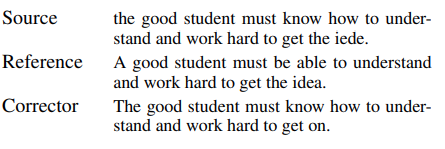
\includegraphics[width=.5\textwidth]{usim1.png}
    \end{center}
\end{frame}


\section{Comparison}


\begin{frame}
\frametitle{UCCA vs. UD}

    \begin{minipage}[t]{.17\textwidth}
      \onslide<2->{
        \fbox{Many formal differences.}
      }
    \end{minipage}
    \begin{minipage}{.5\textwidth}
        \scalebox{.77}{
\begin{tikzpicture}[level distance=2cm, sibling distance=25mm, ->, draw=Indigo, thick]
    \node[anchor=west,font=\bf\sffamily\LARGE,Indigo] at (-3,0) {UCCA};
    \node (ROOT) [fill=Indigo, circle] {}
      child {node (After) {After} edge from parent node[left] {L\;}}
      child {node (graduation) [fill=Indigo, circle] {}
      {
        child {node {graduation} edge from parent node[left] {P}}
      } edge from parent node[left] {H} }
      child {node {,} edge from parent node[right] {U}}
      child {node (moved) [fill=Indigo, circle] {}
      {
        child {node (Daniel) {Daniel} edge from parent node[left] {A}}
        child {node {moved} edge from parent node[left] {P}}
        child {node [fill=Indigo, circle] {}
        {
          child {node {to} edge from parent node[left] {R}}
          child {node {Copenhagen} edge from parent node[left] {C}}
        } edge from parent node[left] {A} }
      } edge from parent node[right] {H} }
      ;
    \draw[dashed,->] (graduation) to node [auto] {A} (Daniel);
\end{tikzpicture}
        }
    \end{minipage}
    \begin{minipage}{.2\textwidth}
      \onslide<3->{
        \fbox{What about \textit{content}?}
        \vspace{4cm}
      }
    \end{minipage}
    
    {\color{DarkBlue}\bf\sffamily\Large UD}
    
    \vspace{-14mm}
    
    \rmfamily
    \begin{dependency}[text only label, edge style={-{Latex[length=2mm]}, color=DarkBlue, thick},
                       label style={above, color=DarkBlue, font=\bf\ttfamily}, font=\small]
    \begin{deptext}[column sep=.8em,ampersand replacement=\^]
    After \^ graduation \^ , \^ Daniel \^ moved \^ to \^ Copenhagen \\
    \end{deptext}
        \depedge{2}{1}{case}
        \depedge{2}{3}{punct}
        \depedge{5}{4}{nsubj}
        \depedge[edge end x offset=-2pt]{5}{2}{obl}
        \depedge{7}{6}{case}
        \deproot[edge unit distance=2.5ex]{5}{root}
        \depedge{5}{7}{obl}
    \end{dependency}
\end{frame}


\begin{frame}
\frametitle{Assimilating the Graph Structures}

\begin{minipage}{.04\textwidth}
\color{DarkBlue} UD
\end{minipage}
\only<-2>{
\begin{minipage}{.45\textwidth}
  \centering
  \scalebox{.6}{
    \begin{dependency}[text only label, edge style={color=DarkBlue},
                       label style={above, color=DarkBlue, font=\bf\ttfamily}, font=\small]
    \begin{deptext}[column sep=.8em,ampersand replacement=\^]
    After \^ graduation \^ , \^ Daniel \^ moved \^ to \^ Copenhagen \\
    \end{deptext}
        \depedge{2}{1}{case}
        \depedge{2}{3}{punct}
        \depedge{5}{4}{nsubj}
        \depedge[edge end x offset=-2pt]{5}{2}{obl}
        \depedge{7}{6}{case}
        \deproot[edge unit distance=2.5ex]{5}{root}
        \depedge{5}{7}{obl}
    \end{dependency}
    }
\end{minipage}
\begin{minipage}{.02\textwidth}
\Rightarrow
\end{minipage}
\begin{minipage}{.4\textwidth}
  \centering
  \scalebox{.55}{\convertedudgraduation}
\end{minipage}
}
\only<3->{
\begin{minipage}{.9\textwidth}
  \centering
  \scalebox{.9}{\convertedudgraduation}
\end{minipage}
}

\pause
\vfill

Evaluate by matching edges \citep*{hershcovich2019content}.

\pause
\vfill

\begin{minipage}{.5\textwidth}
\scalebox{.7}{
\begin{tikzpicture}[level distance=17mm, sibling distance=25mm, ->, draw=Indigo, thick]
    \node[anchor=west,font=\sffamily\LARGE,Indigo] at (-4,0) {UCCA};
    \node (ROOT) [fill=Indigo, circle] {}
      child {node (After) {After} edge from parent node[left] {L\;}}
      child {node (graduation) [fill=Indigo, circle] {}
      {
        child {node {graduation} edge from parent node[left] {P}}
      } edge from parent node[left] {H} }
      child {node {,} edge from parent node[right] {U}}
      child {node (moved) [fill=Indigo, circle] {}
      {
        child {node (Daniel) {Daniel} edge from parent node[left] {A}}
        child {node {moved} edge from parent node[left] {P}}
        child {node [fill=Indigo, circle] {}
        {
          child {node {to} edge from parent node[left] {R}}
          child {node {Copenhagen} edge from parent node[left] {C}}
        } edge from parent node[left] {A} }
      } edge from parent node[right] {H} }
      ;
    \draw[dashed,->] (graduation) to node [auto] {A} (Daniel);
\end{tikzpicture}
}
\end{minipage}
\pause
\begin{minipage}[b]{.4\textwidth}
    \large
    \begin{tabular}{c|c|c}
        \textbf{P} & \textbf{R} & \textbf{F1} \\ \hline
        $\frac89=89\%$ & $\frac8{10}=80\%$ & 84\%
    \end{tabular}
    \vspace{1cm}
\end{minipage}
\end{frame}


\begin{frame}
\frametitle{Scenes and non-Scenes, Relations and Participants}
\begin{flushright}
\scalebox{.9}{
\begin{tikzpicture}[level distance=15mm, sibling distance=21mm, ->, draw=Indigo, thick]
    \node[anchor=west,font=\sffamily\LARGE,Indigo] at (-4,0) {UCCA};
    \node (ROOT) [fill=Indigo, circle] {}
      child {node (After) {After} edge from parent node[above] {L\;}}
      child {node (graduation) [fill=Indigo, circle] {}
      {
        child {node {graduation} edge from parent [Indigo] node[left] {P}}
      } edge from parent [alt=<2>{red}{}] node[left] {H} }
      child {node {,} edge from parent node[right] {U}}
      child {node (moved) [fill=Indigo, circle] {}
      {
        child {node (Daniel) {Daniel} edge from parent [alt=<3>{red}{Indigo}] node[above] {A}}
        child {node {moved} edge from parent [Indigo] node[left] {P}}
        child {node [fill=Indigo, circle] {}
        {
          child {node {to} edge from parent [Indigo] node[left] {R}}
          child {node {Copenhagen} edge from parent [Indigo] node[right] {C}}
        } edge from parent [alt=<3>{red}{Indigo}] node[right] {A} }
      } edge from parent [alt=<2>{red}{}] node[above] {H} }
      ;
    \draw[dashed,->] (graduation) to node [auto] {A} (Daniel);
\end{tikzpicture}
}
\end{flushright}

\vspace{-13mm}

{\color{DarkBlue}\Large\sffamily Converted UD}

\vspace{-1mm}

\scalebox{.9}{\convertedudgraduation}
\end{frame}


\begin{frame}
\frametitle{Multi-word Expressions}

\begin{flushright}
\scalebox{.9}{
\begin{tikzpicture}[level distance=15mm, sibling distance=28mm, ->, draw=Indigo, thick,
  level 2/.style={sibling distance=16mm}]
  \tikzstyle{word} = [color=black]
    \node[anchor=west,font=\sffamily\LARGE,Indigo] at (-4,0) {UCCA};
    \node (ROOT) [fill=Indigo, circle] {}
      child {node (They) [word] {They} edge from parent node[above] {A}}
      child {node [word] {thought} edge from parent node[left] {P}}
      child {node (abouttakingashortbreak) [fill=Indigo, circle] {}
      {
        child {node [word] {about} edge from parent [Indigo] node[left] {R}}
        child {node (takingabreak) [fill=Indigo, circle] {}
        {
          child {node [word] {taking} edge from parent [alt=<3>{red}{Indigo}] node[above] {F}}
          child {node [word] {a} edge from parent [alt=<3>{red}{Indigo}] node[right] {F}}
          child {node [word] (short) {short} edge from parent[draw=none]}
          child {node [word] {break} edge from parent [alt=<3>{red}{Indigo}] node[right] {C}}
        } edge from parent [Indigo] node[right] {P} }
      } edge from parent node[above] {A} }
      ;
    \draw[bend left,dashed,->] (abouttakingashortbreak) to node [auto] {A} (They);
    \draw[bend left,->] (abouttakingashortbreak) to node [auto] {D} (short);
\end{tikzpicture}
}
\end{flushright}

\vspace{-12mm}

\only<1>{
    {\color{DarkBlue}\Large\sffamily UD}

     \begin{dependency}[line width=1.5pt]
        \begin{deptext}[column sep=1.5em,ampersand replacement=\^,font=\rmfamily]
       They \^ thought \^ about \^ taking \^ a \^ short \^ break \\
         \end{deptext}
        \deproot[draw=DarkBlue]{2}{root}
        \depedge[draw=DarkBlue]{2}{1}{nsubj}
        \depedge[edge start x offset=-4pt,draw=DarkBlue]{2}{4}{advcl}
        \depedge[draw=DarkBlue]{4}{3}{mark}
        \depedge[draw=DarkBlue]{4}{7}{dobj}
        \depedge[draw=DarkBlue]{7}{5}{det}
        \depedge[draw=DarkBlue]{7}{6}{amod}
    \end{dependency}
}
\only<2->{
  \vspace{-16mm}
    
  {\color{DarkBlue}\Large\sffamily Converted UD}
  
  \scalebox{.9}{
  \begin{tikzpicture}[level distance=17mm, sibling distance=28mm, ->, draw=DarkBlue, thick,
      every node/.append style={sloped,anchor=south,auto=false,font=\scriptsize},
      level 2/.style={sibling distance=19mm},
      edge from parent path={(\tikzparentnode.center) -- (\tikzchildnode.north)}]
    \tikzstyle{word} = [font=\rmfamily,color=black]
    \node (ROOT) [fill=DarkBlue, circle] {}
      child {node (They) [word] {They} edge from parent node {nsubj}}
      child {node [word] {thought} edge from parent node {head}}
      child {node (abouttakingashortbreak) [fill=DarkBlue, circle] {}
      {
        child {node [word] {about} edge from parent node {mark}}
        child {node (takingabreak) [fill=DarkBlue, circle] {}
        {
          child {node [word] {taking} edge from parent node {head}}
          child {node [word] {a} edge from parent node {det}}
          child {node [word] (short) {short} edge from parent node {\;amod}}
          child {node [word] {break} edge from parent node {head}}
        } edge from parent node {dobj} }
      } edge from parent node {advcl} }
      ;
  \end{tikzpicture}
  }
}
\end{frame}


\begin{frame}
\frametitle{Linkage between Scenes}

\begin{flushright}    
    \scalebox{.8}{
    \begin{tikzpicture}[level distance=15mm, sibling distance=39mm, ->, draw=Indigo, thick,
  level 2/.style={sibling distance=16mm},
  every circle node/.append style={fill=Indigo}]
  \tikzstyle{word} = [color=black]
    \node[anchor=west,font=\sffamily\LARGE,Indigo] at (-6,0) {UCCA};
      \node (ROOT) [circle] {}
        child {node [circle] {}
        {
          child {node [word] {From} edge from parent [Indigo] node[left] {R}}
          child {node [word] {the} edge from parent [Indigo] node[left] {E}}
          child {node [word] {{\color{white}F}\color{black}moment} edge from parent [Indigo] node[right] {C}}
        } edge from parent [alt=<2>{red}{}] node[above] {L} }
        child {node [circle] {}
        {
          child {node [word] {you{\color{white}k}} edge from parent node[left] {A}}
          child {node [word] {{\color{white}y}enter} edge from parent node[right] {P}}
        } edge from parent node[left] {H} }
        child {node [circle] {}
        {
          child {node (comma) [word] {,} edge from parent [draw=none]}
          child {node [word] {you{\color{white}k}} edge from parent node[left] {A}}
          child {node [word] {{\color{white}y}know} edge from parent node[right] {S}}
        } edge from parent node[above] {H} }
        ;
      \draw[->] (ROOT) to node [right] {U} (comma);
    \end{tikzpicture}
    }
\end{flushright}

    {\color{DarkBlue}\Large\sffamily UD}
    
    \vspace{-5mm}
    
    \begin{dependency}[line width=1.5pt]
        \begin{deptext}[column sep=1.5em,ampersand replacement=\^,font=\rmfamily]
        From \^ the \^ moment \^ you \^ enter \^ , \^ you \^ know \\
        \end{deptext}
        \depedge[draw=DarkBlue]{3}{1}{case}
        \depedge[draw=DarkBlue]{3}{2}{det}
        \depedge[draw=DarkBlue]{8}{3}{obl}
        \depedge[draw=DarkBlue]{3}{5}{acl}
        \depedge[draw=DarkBlue,edge start x offset=-5pt]{5}{4}{nsubj}
        \depedge[draw=DarkBlue]{8}{6}{punct}
        \depedge[draw=DarkBlue,edge start x offset=-10pt]{8}{7}{nsubj}
        \deproot[draw=DarkBlue]{8}{root}
    \end{dependency}
\end{frame}

\begin{frame}
\frametitle{Comparison by Conversion: Reverse-Engineering UCCA from Syntax and Lexical Semantics}

Complement syntax with \textit{lexical} semantics to make up for differences
\citep{hershcovich-et-al-2020-comparison}.

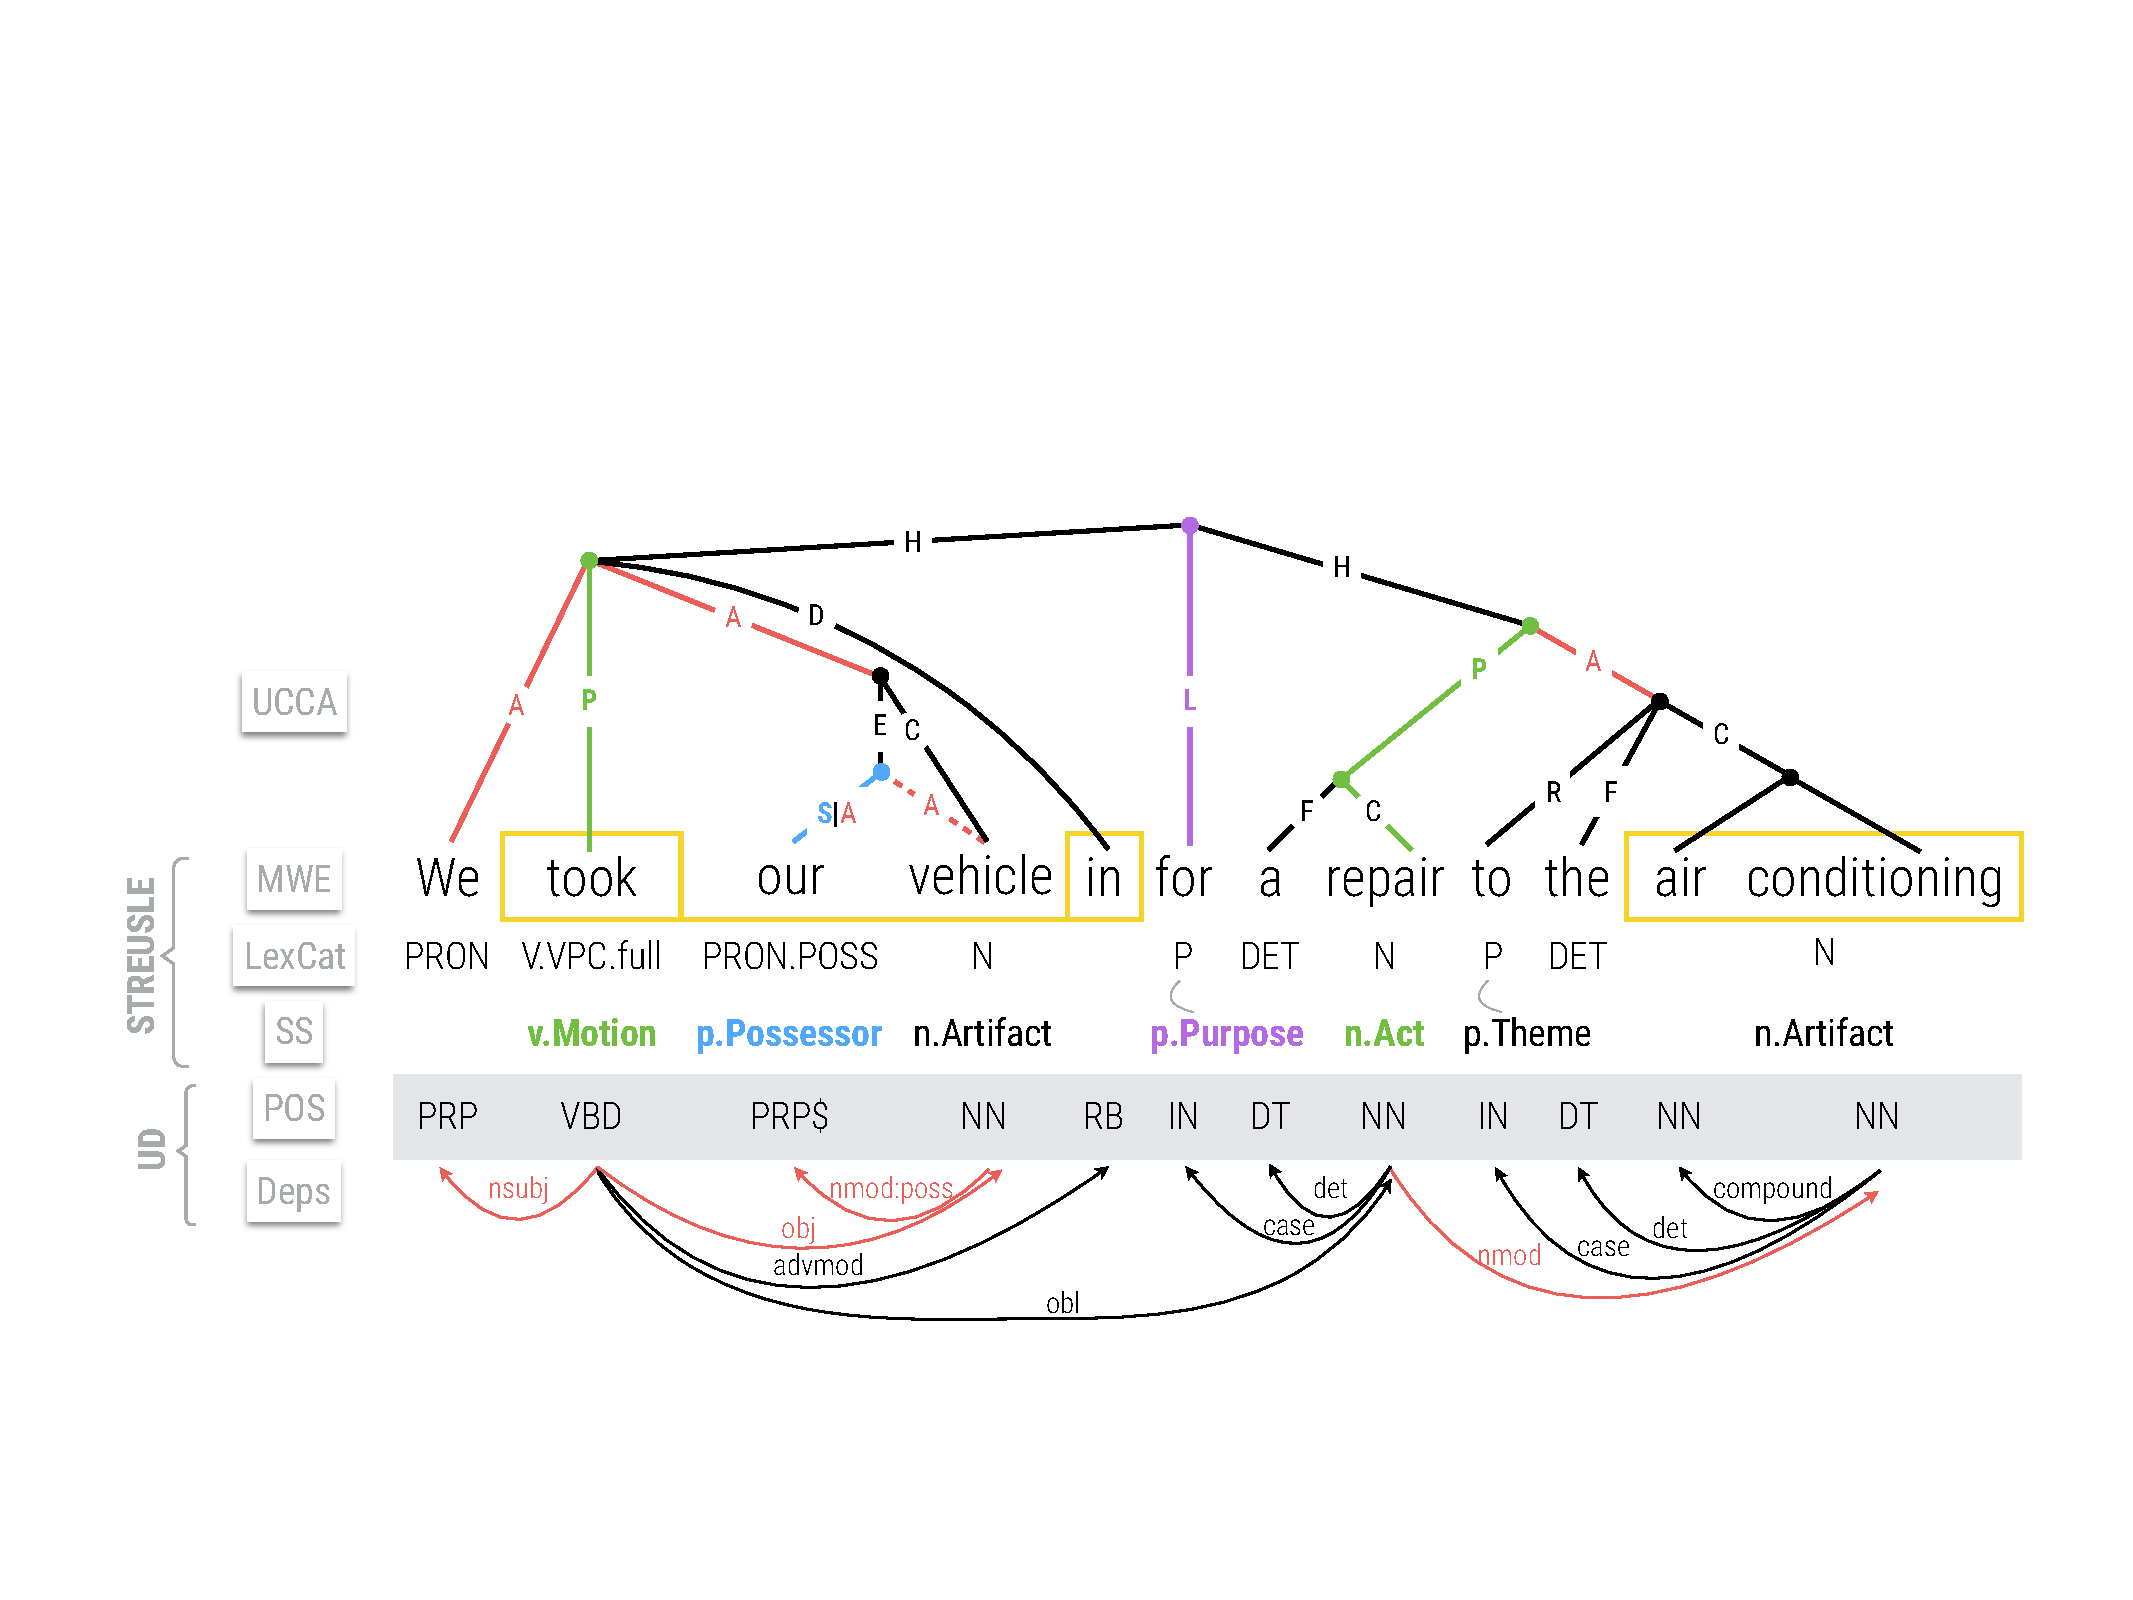
\includegraphics[width=\textwidth]{ex-ucca-streusle.pdf}
\end{frame}

\section*{}

\begin{frame}
\frametitle{Conclusion}
\begin{itemize}
 \item Meaning representation is valuable for language understanding.\pause
 \item Transition-based parsers excel across frameworks and languages.\pause
 \item Cross-framework unification by multi-task and linguistic analysis.
\end{itemize}

\vfill
\begin{flushright}
Thanks!
\end{flushright}

\end{frame}

\begin{frame}[allowframebreaks]
\frametitle{References}
\bibliographystyle{plainnat}
\tiny\bibliography{references,mrp,anthology}
\end{frame}

\begin{frame}
\frametitle{Structural Properties}
\noindent
\centering
\begin{minipage}{.5\linewidth}{\centering
(1) {\color{blue} non-terminal nodes}

\scalebox{.8}{
  \begin{tikzpicture}[level distance=12mm, sibling distance=16mm, ->, thick,
      every node/.append style={midway},
      edge from parent/.append style={nodes={font=\scriptsize}}]
    \node (ROOT) [fill=blue, circle] {}
      child {node [fill=blue, circle] {}
      {
        child {node {John} edge from parent node[left] {C}}
        child {node {and} edge from parent node[left] {N}}
        child {node {Mary} edge from parent node[right] {C}}
      } edge from parent node[left] {A} }
      child {node {went} edge from parent node[left] {P}}
      child {node {home} edge from parent node[right] {A}}
      ;
  \end{tikzpicture}
  }}
\end{minipage}
\hfill
\begin{minipage}{.48\linewidth}{\centering
(2) {\color{red} discontinuity}

\scalebox{.8}{
  \begin{tikzpicture}[level distance=12mm, sibling distance=2cm, ->, thick,
      every node/.append style={midway},
      edge from parent/.append style={nodes={font=\scriptsize}}]
    \node (ROOT) [fill=black, circle] {}
      child {node {John} edge from parent node[left] {A}}
      child {node [fill=black, circle] {}
      {
      	child {node {gave} edge from parent node[left] {C}}
      	child {node (everything) {everything} edge from parent[white]}
      	child {node {up} edge from parent node[right] {C}}
      } edge from parent node[right] {P} }
      ;
    \draw[bend right,->,red,very thick] (ROOT) to[out=-20, in=180] node [left] {\scriptsize A} (everything);
  \end{tikzpicture}
  }}
\end{minipage}

\vfill
(3) {\color{orange} reentrancy}

\scalebox{.8}{
\begin{tikzpicture}[level distance=14mm, sibling distance=17mm, ->, thick,
    edge from parent/.append style={nodes={font=\scriptsize}}]
    \node (ROOT) [fill=black, circle] {}
      child {node (After) {After} edge from parent node[left] {L\;}}
      child {node (graduation) [fill=black, circle] {}
      {
        child {node {graduation} edge from parent node[left] {P}}
      } edge from parent node[left] {H} }
      child {node {,} edge from parent node[right] {U}}
      child {node (moved) [fill=black, circle] {}
      {
        child {node (John) {John} edge from parent node[left] {A}}
        child {node {moved} edge from parent node[left] {P}}
        child {node [fill=black, circle] {}
        {
          child {node {to} edge from parent node[left] {R}}
          child {node {Copenhagen} edge from parent node[right] {C}}
        } edge from parent node[right] {A} }
      } edge from parent node[right] {H} }
      ;
    \draw[dashed,->,orange,very thick] (graduation) to node [auto] {\scriptsize A} (John);
\end{tikzpicture}}
\end{frame}


\begin{frame}
\frametitle{Data Statistics}
\centering
\def\arraystretch{1.5}
\begin{tabular}{l|r|rrr|r}
    & \multicolumn{1}{c|}{Wiki} & \multicolumn{3}{c|}{20K} & \multicolumn{1}{c}{EWT} \\
    & \multicolumn{1}{c|}{en} & \multicolumn{1}{c}{en} & \multicolumn{1}{c}{fr} & \multicolumn{1}{c|}{de} & \multicolumn{1}{c}{en} \\
    \hline
    \# sentences&5,141&492&492&6,514&3,520 \\
    \# tokens&158,739&12,638&13,021&144,529&51,042 \\
    \hline
    \# {\color{blue} non-terminal nodes}&62,002&4,699&5,110&51,934&18,156 \\
    \% {\color{red}discontinuous}&1.71&3.19&4.64&8.87&3.87 \\
    \% {\color{orange}reentrant}&1.84&0.89&0.65&0.31&0.83 \\
    \hline
    \# edges&208,937&16,803&17,520&187,533&60,739 \\
    \% primary&97.40&96.79&97.02&97.32&97.32 \\
    \% remote&2.60&3.21&2.98&2.68&2.68
\end{tabular}
\end{frame}


\begin{frame}
\frametitle{Evaluation}
\begin{adjustbox}{frame,scale=.75,center}
    \begin{tikzpicture}[level distance=12mm, sibling distance=15mm, ->,
        every circle node/.append style={fill=black},
        edge from parent/.append style={nodes={font=\scriptsize}},
        edge from parent path={(\tikzparentnode.center) -- (\tikzchildnode.north)}]
      \tikzstyle{word} = [font=\rmfamily,color=black]
      \node at (0,.7) {True (human-annotated) graph};
      \node (ROOT) at (0,0) [circle] {}
        child {node (After) [word] {After} edge from parent node[left] {L}}
        child {node (graduation) [circle] {}
        {
          child {node [word] {graduation} edge from parent node[left] {P}}
        } edge from parent node[left] {H} }
        child {node [word] {,} edge from parent node[right] {U}}
        child {node (moved) [circle] {}
        {
          child {node (John) [word] {John} edge from parent node[left] {A}}
          child {node [word] {moved} edge from parent node[left] {P}}
          child {node [circle] {}
          {
            child {node [word] {to} edge from parent node[left] {R}}
            child {node [word] {Copenhagen} edge from parent node[right] {C}}
          } edge from parent node[right] {A} }
        } edge from parent node[right] {H} }
        ;
      \draw[dashed,->] (graduation) to node [auto] {\scriptsize A} (John);
      \node at (8,.7) {Automatically predicted graph for the same text};
      \node (ROOT_) at (7,0) [circle] {}
        child {node (After_) [word] {After} edge from parent node[left] {L}}
        child {node (graduation_) [circle] {}
        {
          child[alt=<2>{red}{}] {node [word] {graduation} edge from parent node[left] {S}}
        } edge from parent node[left] {H} }
        child {node [word] {,} edge from parent node[right] {U}}
        child {node (moved) [circle,xshift=3mm,yshift=-7mm] {}
        {
          child {node (John_) [word] {John} edge from parent node[left] {A}}
          child {node [word] {moved} edge from parent node[left] {P}}
          child[alt=<2>{red}{}] {node [word] {to} edge from parent node[left] {F}}
          child[alt=<2>{red}{}] {node (Copenhagen_) [word] {Copenhagen} edge from parent node[right] {A}}
        } edge from parent node[right] {H} }
        ;
      \draw[dashed,->] (graduation_) to node [auto] {\scriptsize A} (John_);
      \draw[bend left,dashed,->,alt=<2>{red}{}] (graduation_) to[in=90] node [auto] {\scriptsize A} (Copenhagen_);
    \end{tikzpicture}
\end{adjustbox}
\vfill

\begin{enumerate}
  \item Match primary edges between the graphs by terminal yield and label.
  \item Calculate \textbf{precision, recall and F1} scores.
  \item Repeat for remote edges.
\end{enumerate}

\pause
\vfill
\begin{adjustbox}{center}
    \begin{tabular}{c|c|c}
        \multicolumn{3}{l}{Primary} \\
        \textbf{P} & \textbf{R} & \textbf{F1} \\ \hline
        $\frac69=67\%$ & $\frac6{10}=60\%$ & 64\%
    \end{tabular}
    \hspace{1cm}
    \begin{tabular}{c|c|c}
        \multicolumn{3}{l}{Remote} \\
        \textbf{P} & \textbf{R} & \textbf{F1} \\ \hline
        $\frac12=50\%$ & $\frac11=100\%$ & 67\%
    \end{tabular}
\end{adjustbox}
\end{frame}

\end{document}
